%!TEX root = main.tex
\chapter{Dataset}
På de følgende sider vil vi gennnemgå vores dataset. Vi vil vise de basale statistikker over det pågældende data vi har arbejdet med og gennemgå afvigelser. Vi vil også gennemgå hvordan vi forholder os til disse afvigelser og hvordan vi lavede datacleaning. \\
Til sidst vil vi runde afsnittet af med en del-konlusion. 

Vores data stammer fra Sony's Lifelog\cite{sonyLifeLog} som, navnet antyder, er en mobil Lifelog app som logger ens aktiviteter i løbet af dagen. Heri logger den bla. aktivitet i apps og geolokation. Vores dataset stammer fra denne app, indsamlet fra Sony mobiltelefoner verden over. % over 3 måneder\footnote{September 2015 - November 2015} fordelt på 80 lande. 

%Vi har valgt at dele datasættet op i to dele, for overblikkets skylde: En \textbf{geolokation del} og en \textbf{app og homophily del}.

%\section{Geolokation del}

Datasættet beskriver geolokationerne for hvor en bruger har været. Det beskriver præcis hvor, hvornår og hvor længe brugeren har været det pågældende sted. Hver gang brugeren skifter lokation (defineret ud fra latitude og longitude), bliver der logget en lokationsopdatering med følgende oplysninger:
\begin{enumerate}
\item \texttt{\textbf{timestamp\_seen}}\\Millisekunder siden brugerens systems epoch, da den pågældende lokations opdatering bliver logget. 
\item \texttt{\textbf{id}}\\Lokations id repræsenteret som en streng. 
\item \texttt{\textbf{useruuid}}\\Brugerens unikke id repræsenteret som en streng
\item \texttt{\textbf{start\_time}}\\Tid for hvornår brugeren går ind i en lokation. Repræsenteret som ISO8601 time stamp med timezone
\item \texttt{\textbf{end\_time}}\\Tid for hvornår brugeren går ud af en lokation. Repræsenteret som ISO8601 time stamp med timezone
\item \texttt{\textbf{name}}\\Navnet på byen hvor brugeren befinder sig, når lokations opdateringen bliver logget
\item \texttt{\textbf{area}}\\Navnet på området hvor brugeren befinder sig, når lokations opdateringen bliver logget. F.eks. Skåne i Sverige
\item \texttt{\textbf{country}}\\Navnet på landet hvor brugeren befinder sig, når lokations opdateringen bliver logget.
\item \texttt{\textbf{region}}\\Navnet på regionen hvor brugeren befinder sig, når lokations opdateringen bliver logget. F.eks. Europa
\item \texttt{\textbf{latitude}}\\Latitude for lokationen. Latitude har en præcition på ca 15 cifre, hvilket svarer til 0.1 nanometer \textcolor{red}{[KILDE!!!]}. Denne præcition er skal man dog ikke tage så højtidligt, da de fleste mobil GPS'er har en fejl margen på maks 30 meter \cite{NAV:8292634}.  
\item \texttt{\textbf{longitude}}\\Longitude for lokationen. Latitude har en præcition på ca 15 cifre, hvilket svarer til 0.1 nanometer. Vedr. præcition, gælder det samme som ved latitude
\item \texttt{\textbf{altitude}}\\Altitude repræsenteret i mm. Dette bliver beregnet af telefonens gyroskop samt GPS
\item \texttt{\textbf{accuracy}}\\Accuracy repræsenteret i mm. Accuracy er hvor nøjagtigt man kan regne med GPS'en er i den pågældene lokations opdatering. Værdien fortæller at brugeren med 68\% sikkerhed er i pågældende sted, indenfor denne distance som accuracy er \cite{android_accuracy}. Jo lavere værdi, jo bedre. Dette styres af telefonens styresystem og GPS
\item \texttt{\textbf{devices}}\\Devices er repræsentet som et array med name, type og id. Type er hvilken type device (f.eks. Phone), name er navnet på det device og id er devices unikke id. 
\end{enumerate}

Nogle af overstående oplysninger er ikke relevante for vores problemstilling. Dette gør vi kan skære disse fra og vi ender dermed at have følgende oplysninger (fra nu af kaldt  attributter) at arbejde med: 

\begin{itemize}
\item \texttt{useruuid}
\item \texttt{start\_time}
\item \texttt{end\_time}
\item \texttt{country}
\item \texttt{latitude}
\item \texttt{longitude}
\end{itemize}

Disse oplysinger har vi valgt, da de mere eller mindre er vigtige eller interssante i forhold til vores problemstilling. \texttt{useruuid} er vigtig for at kunne skelne brugerene fra hinanden, \texttt{start\_time} og \texttt{end\_time} er vigtige, da de fortæller hvornår og hvor længe brugeren har været i den pågældende lokation. \texttt{country} er til nemt at kunne filtrere brugerene. \texttt{latitude} og \texttt{longitude} er meget væsentlige, da de fortæller det mest vigtigste, nemlig hvilken lokation brugeren befinder sig i. \texttt{accuracy} kan fortælle os i for høj grad vi kan bruge den pågældene lokationsopdatering.  


Vi har kigget på test data som er et sub-sæt af production data. Dette test data, er fra en specifik periode og med specifikke brugere. Efter dette sub-sæt, har vi kigget på hele production data. Vi vil beskrive hvordan henholdsvis test data og production data ser ud mht. distributioner mm. 

\section{Test data}
Dette data's periode strakte sig over 3 måneder: september - november 2015. 
Henover denne periode blev der indsamlet 2,665,893 lokations opdateringer fordelt på 1,586 brugere. Disse brugere er alle Sony medarbejdere rundt om i verdenen. Dette betyder at de har nogle naturlige samlingssteder som er Sony relaterede, såsom Sonys kontorer rundt i diverse lande. \textcolor{red}{figur af kort eller henvisning?}
Dette har i højgrad en indvirkning på vores hvordan dataet ser ud, hvilket vi vender tilbage til. 

I Table \ref{tab:stat_geo_p1} ses statistic summary af \texttt{accuracy}.
Vi kan se i tabellen, at der er nogle ugyldige værdier for accuracy. Disse ugyldige værdier viser sig i form af negative værdier. 
Ud af de mange lokations opdateringer er der kun 20 hvor accuracy er negativ hvilket svarer til knapt en 1,000 del procent. 
\begin{table}[H]
        \centering
        \small
        \setlength\tabcolsep{2pt}
        \begin{tabular}{|c|c|c|}
            \hline
                         & Accuracy (mm)          \\[0pt]% compensate for extrarowheight
            \hline
                 Min     &  -2,147,483,500             \\
            \hline
                 Max     &  500,000                \\
            \hline
                 Mean    & 35,249                      \\
            \hline
                Std. dev.   & 3,672,390                \\
            \hline
        \end{tabular}
        \caption{Statistic summary of dataset in test periode} %add this between 'caption' and '{...' for new text in listing of tables: [New caption text only for listing of tables]
        \label{tab:stat_geo_p1}
\end{table}

Da accuracy påvirker latitude og longitude, som er vores vigtigste attribut, så fjerner vi de opdateringer hvor acuracy er negativ. Herudover fjerner vi også de lokations opdateringer hvor accuracy er over 55.000 (55m). Vores binning svare maksimalt til 111m. Da accuracy fortæller at brugeren med 68\% sikkerhed er i pågældende sted, indenfor denne distance som accuracy er, vælger vi derfor 55m som er halvdelen af den maksimale længde, vores cell kan være. Det gør, at vi med 68\% sikkerhed ved, at brugeren er i den pågældende binning, med den forudsætning, at brugeren er står præcis i midten af cellen. Dette er dog en forudsætning, som vi ikke kan gå ud fra er gældene. Dog synes vi, dette er den bedste måde at sætte grænsen for accuracy på. 
Se mere i section \ref{ssec:binning}, s. \pageref{ssec:binning}, ang. hvordan binning er defineret og i dicussion for vores udfordringer mht. binning og cell size. 

Efter dette, så quantilerne af accuracy ud som man kan se på Tabel \ref{tab:acc_quantiles}. 
 \begin{table}[htbp]
        \centering
        \small
        \setlength\tabcolsep{2pt}
        \begin{tabular}{|c|c|c|}
            \hline
                         & Accuracy      \\[0pt]
            \hline
                 Min     &  3,000       \\
            \hline
                 Q1      &  9,000   \\
            \hline
                 Median  &  20,000    \\
            \hline
                 Mean    &  22,565.72    \\
            \hline
                 Q3      &  35,541      \\
            \hline
                 Max &  55,000   \\
            \hline
                 IQR     &   26,541     \\
            \hline
                Std. dev.  &  14,669.72   \\
            \hline
        \end{tabular}
        \caption{Quantiles of accuracy after cleaning} %add this between 'caption' and '{...' for new text in listing of tables: [New caption text only for listing of tables]
        \label{tab:acc_quantiles}
\end{table}

Vi kan se på medianen og mean, at de fleste brugere har lav værdi i accuracy - hvilket er godt! Hvis vi antager at det følger en normalfordeling, kan vi ud fra standard deviation udlede, at 95\% af brugerne har en accuracy mellem 7,896 og 37,235.44. Dette viser at der sandsynligvis er nogle få brugere med meget høje værdier i accuracy, hvor max er 100,000. At det kun er nogle få brugere med høje værdier er godt, da det omvendt betyder at der er mange bruger med lav (og derved god) accuracy. Da vi har gjort at max for accuracy er 100,000, kan vi sagtens bruge disse brugere med høj værdi i accuracy. Hvis man senere skulle bruge en mere fin binning, ville man sagtens kunne gøre dette uden at skulle udelukke alt for meget data, da værdierne for accuracy ligger så fint som de gør.  

Medianen og mean svarer til henholdsvis 23m og 26.89m og 95\% standard deviation er på mellem 6.6m og 47.19m hvilken er en fin accuracy. 


Når vi kigger på hvilke lande der er repræsenteret og i hvilken grad, har vi at gøre med 80 unikke lande. Til at starte med lå dette tal på 74. Det viste sig, at der var en masse lokations opdateringer hvor landet ikke var blevet logget. I disse tilfælde var landet blot repræsenteret med en tom streng. Dette var tilfældet i så stor en del af dataet, at landet med en tom streng, var det andet mest repræsenterede land i dataet med lidt over 500.000 lokations opdateringer. 
Da vi gerne vil kunne sorterer data på baggrund af land, var dette et problem. Dette fik vi løst, ved at udføre omvendt geolokation. For næsten alle de 500.000 lokations opdateringer, var latitude og longitude til stede, så vi kunne ved hjælp af et API\cite{reversegeocode} slå landet op på bagrund af latitude og longitude, og herefter indsætte det i dataet. Dette gjorde vi kun skulle gøre dette én gang, i stedet for at slå landet op hver gang vi kørte vores scripts. Dette ville have været ineffektivt og spild af tid. Derudover havde API'et en grænse hvor hvor mange man kunne slå op i minuttet, hvilket gjorde at det tog en uges tid at slå alle op. Her kørte scriptet 24/7. \\ 
Vores omvendt geolokation gjorde, at vi gik fra over 500,000 lokations opdateringer hvor landet ikke var til stede, til blot 130 lokations opdateringer. I samme omgang fik vi nye lande repræsenteret i dataet, så vi gik fra 74 lande til 80 (inkl. land med tom streng)

Vi kan herefter kigge på, hvordan lokations opdateringerne er distribueret over de fem lande, med højest antal opdateringer. På figur \ref{fig:country_dist} kan vi se at Sverige og Japan topper listen og ay landet med en tom streng er udenfor top 5 (det røg ned blandt den sidste fjerde del).


\begin{figure}[H]
    \hspace*{-1.0cm}
    \centering
    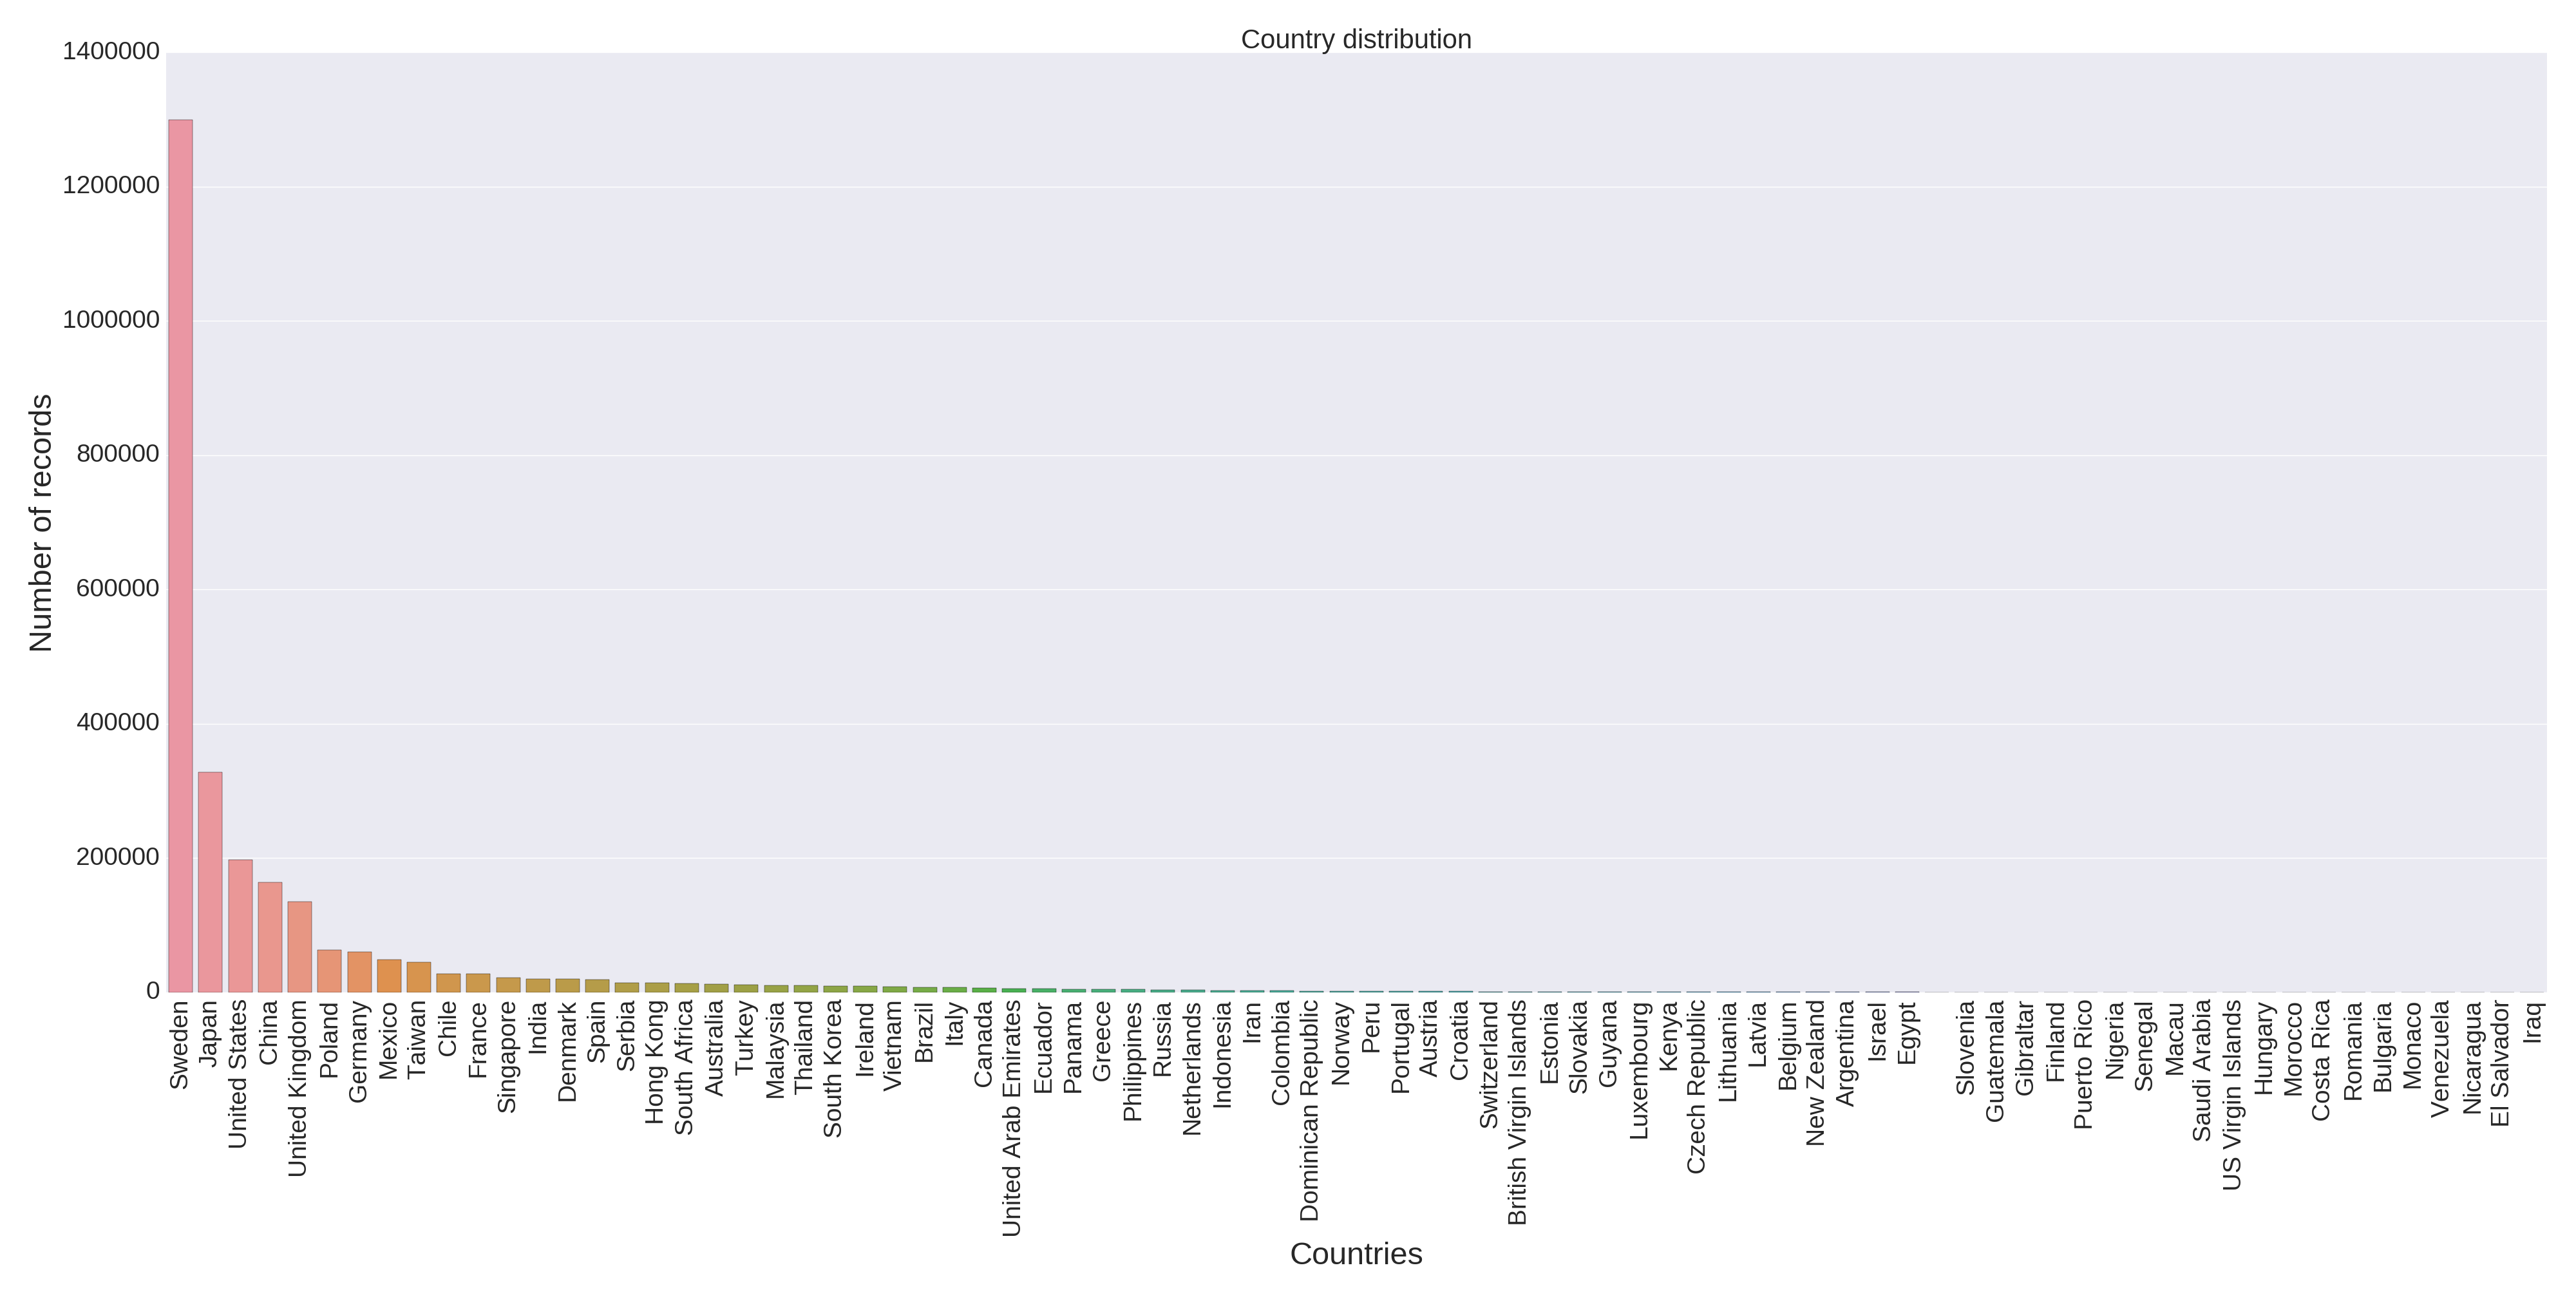
\includegraphics[scale=0.14]{country_distribution}
    \caption{Distribution for number of location updates between the five countries with most updates}
    \label{fig:country_dist}
\end{figure}


At Sverige og Japan er de to størst repræsenterede lande er ikke så mærkeligt, da Sony er et Japansk firma og Sony overtog helt Sony-Ericsson, hvor Ericsson var Svensk. Sony-Ericsson var den gang Sony's mobil mærke, så en stor del af Sony's mobil udvikling ligger stadig i Sverige. Dette kan forsklare hvorfor Sverige har tre gange flere opdateringer end Japan.  

På baggrund af Figure \ref{fig:country_dist}, har vi valgt at gå videre med endten Sverige eller Japan. Derfor vil vi nu sammeligne data for de to lande. 
I Japan er der \numberUsersJapan{} unikke brugere, mens der i Sverige er \numberUsersSweden. De to lande kan have brugere tilfælles, da brugerne principielt kan rejse mellem flere lande og derved have lokations opdateringer i flere lande.  
Af antallet af totale lokations opdateringer har Japan 299,157 opdateringer henover alle tre måneder, mens Sverige har 1,018,781 opdateringer.

Figure \ref{fig:mean_loc_updates_sep-nov} sammenligner gennemsnittet for lokations opdateringer i Japan og Sverige.
\begin{figure}[H]
    \hspace*{-2.2cm}
    \centering
    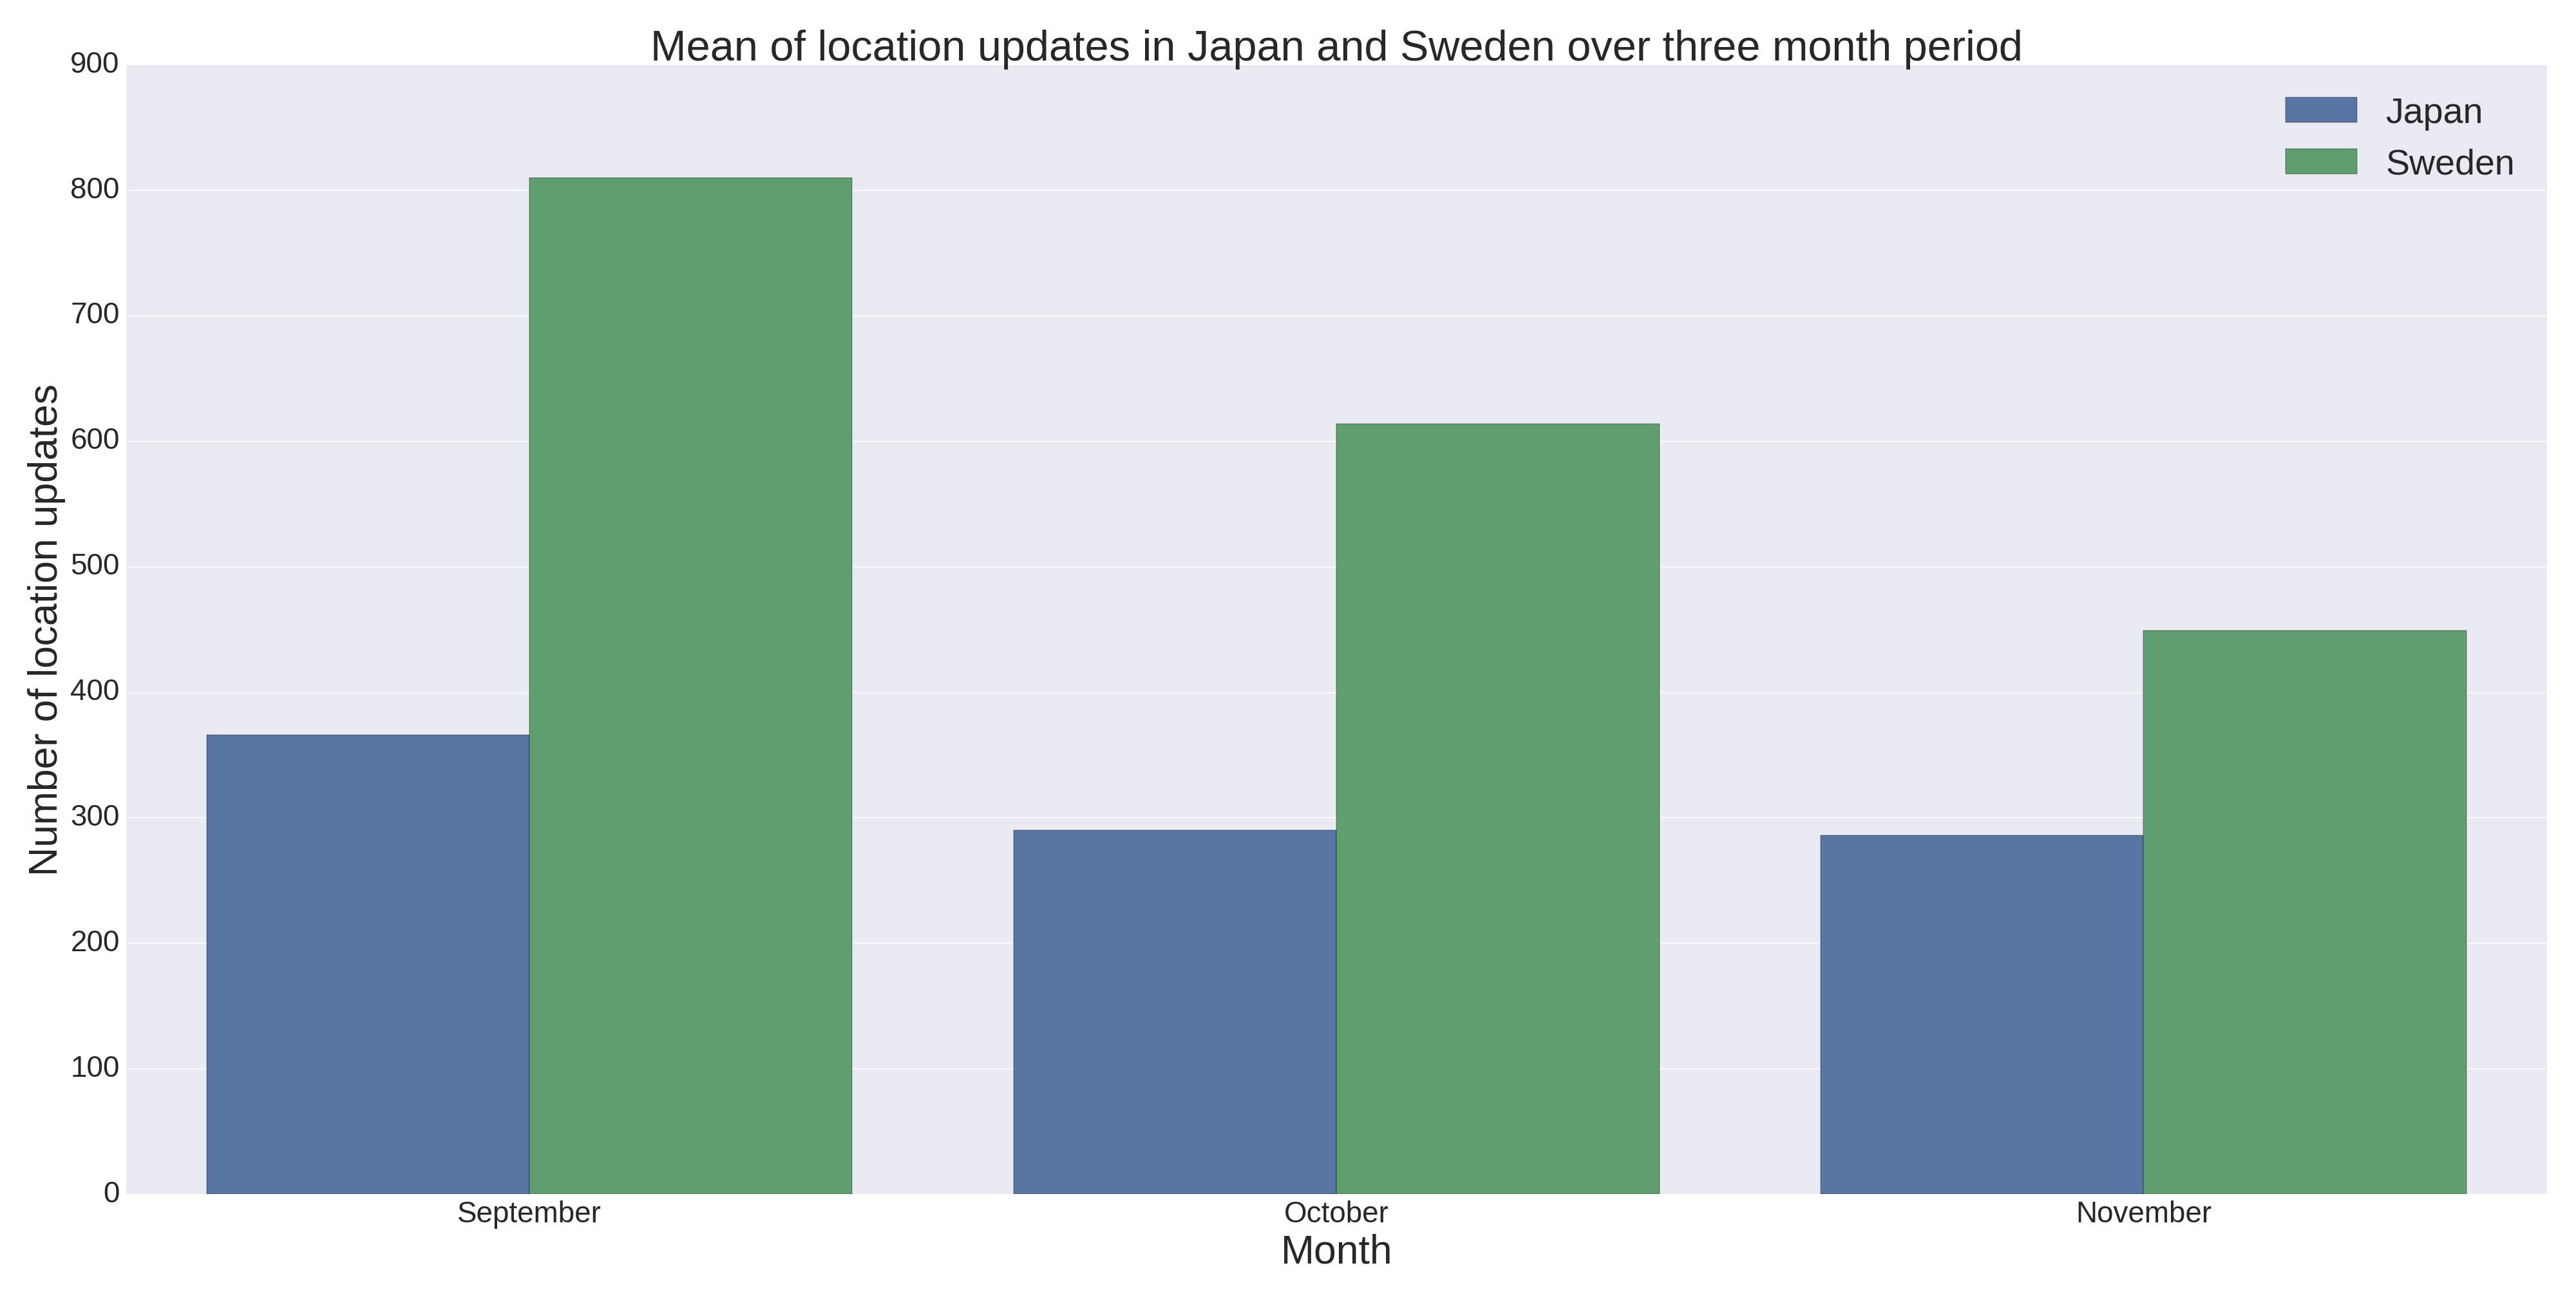
\includegraphics[scale=0.16]{mean_loc_updates_sep-nov}
    \caption{Distribution for mean of location updates for Japan and Sweden}
    \label{fig:mean_loc_updates_sep-nov}
\end{figure}

Vi kan se at Sverige har betydeligt flere opdateringer end Japan i alle tre måneder, hvor landet i September og Oktober endda har dobbelt så mange end Japan. Vi kan også se en nedadgående tendens i begge lande. September har højest antal opdateringer, hvor det herefter går nedad i de to resterende måneder, hvor November for Sverige ligger over 300 opdateringer under September. Selvom tendensen ses tydeligst for Sverige, er den også synlig for Japan. \\
Dette kigger vi nærmere på senere. \textcolor{red}{heatmaps???}

Som der blev nævnt tidligere, er der nogle naturlige samlingssteder for Sverige og Japan, da dataet er for Sony medarbejdere. Disse steder er naturligvis arbejdsrelaterede, såsom Sonys kontorer i de to lande. Vi har fundet frem til to steder i Sverige og et i Japan. Grunden til at dette er væsentligt for os er, at folk selvfølgelig har flere co-occurrences på et arbejdsrelateret sted, end et ikke arbejdsrelateret sted, da man er mange på et forholdvis lille område.\textcolor{red}{kilde?!?!} Derudover er der møder, pauser og andet som også gør at folk har en co-occurrence. Dette lyder meget godt, men det betyder langt fra at folk kender hinanden, fordi de har en co-occurence. Folk møder ofte kolegaer, uden de nødvendigvis kender hinanden. \textcolor{red}{Dette er noget vi beskriver nærmere i ....}

Det er derfor interessant at se, hvor mange af opdateringer for hvert land der ligger indenfor de fundne samlingssteder og hvor mange der ligger udenfor. 

\begin{figure}[H]
    \hspace*{-2.2cm}
    \centering
    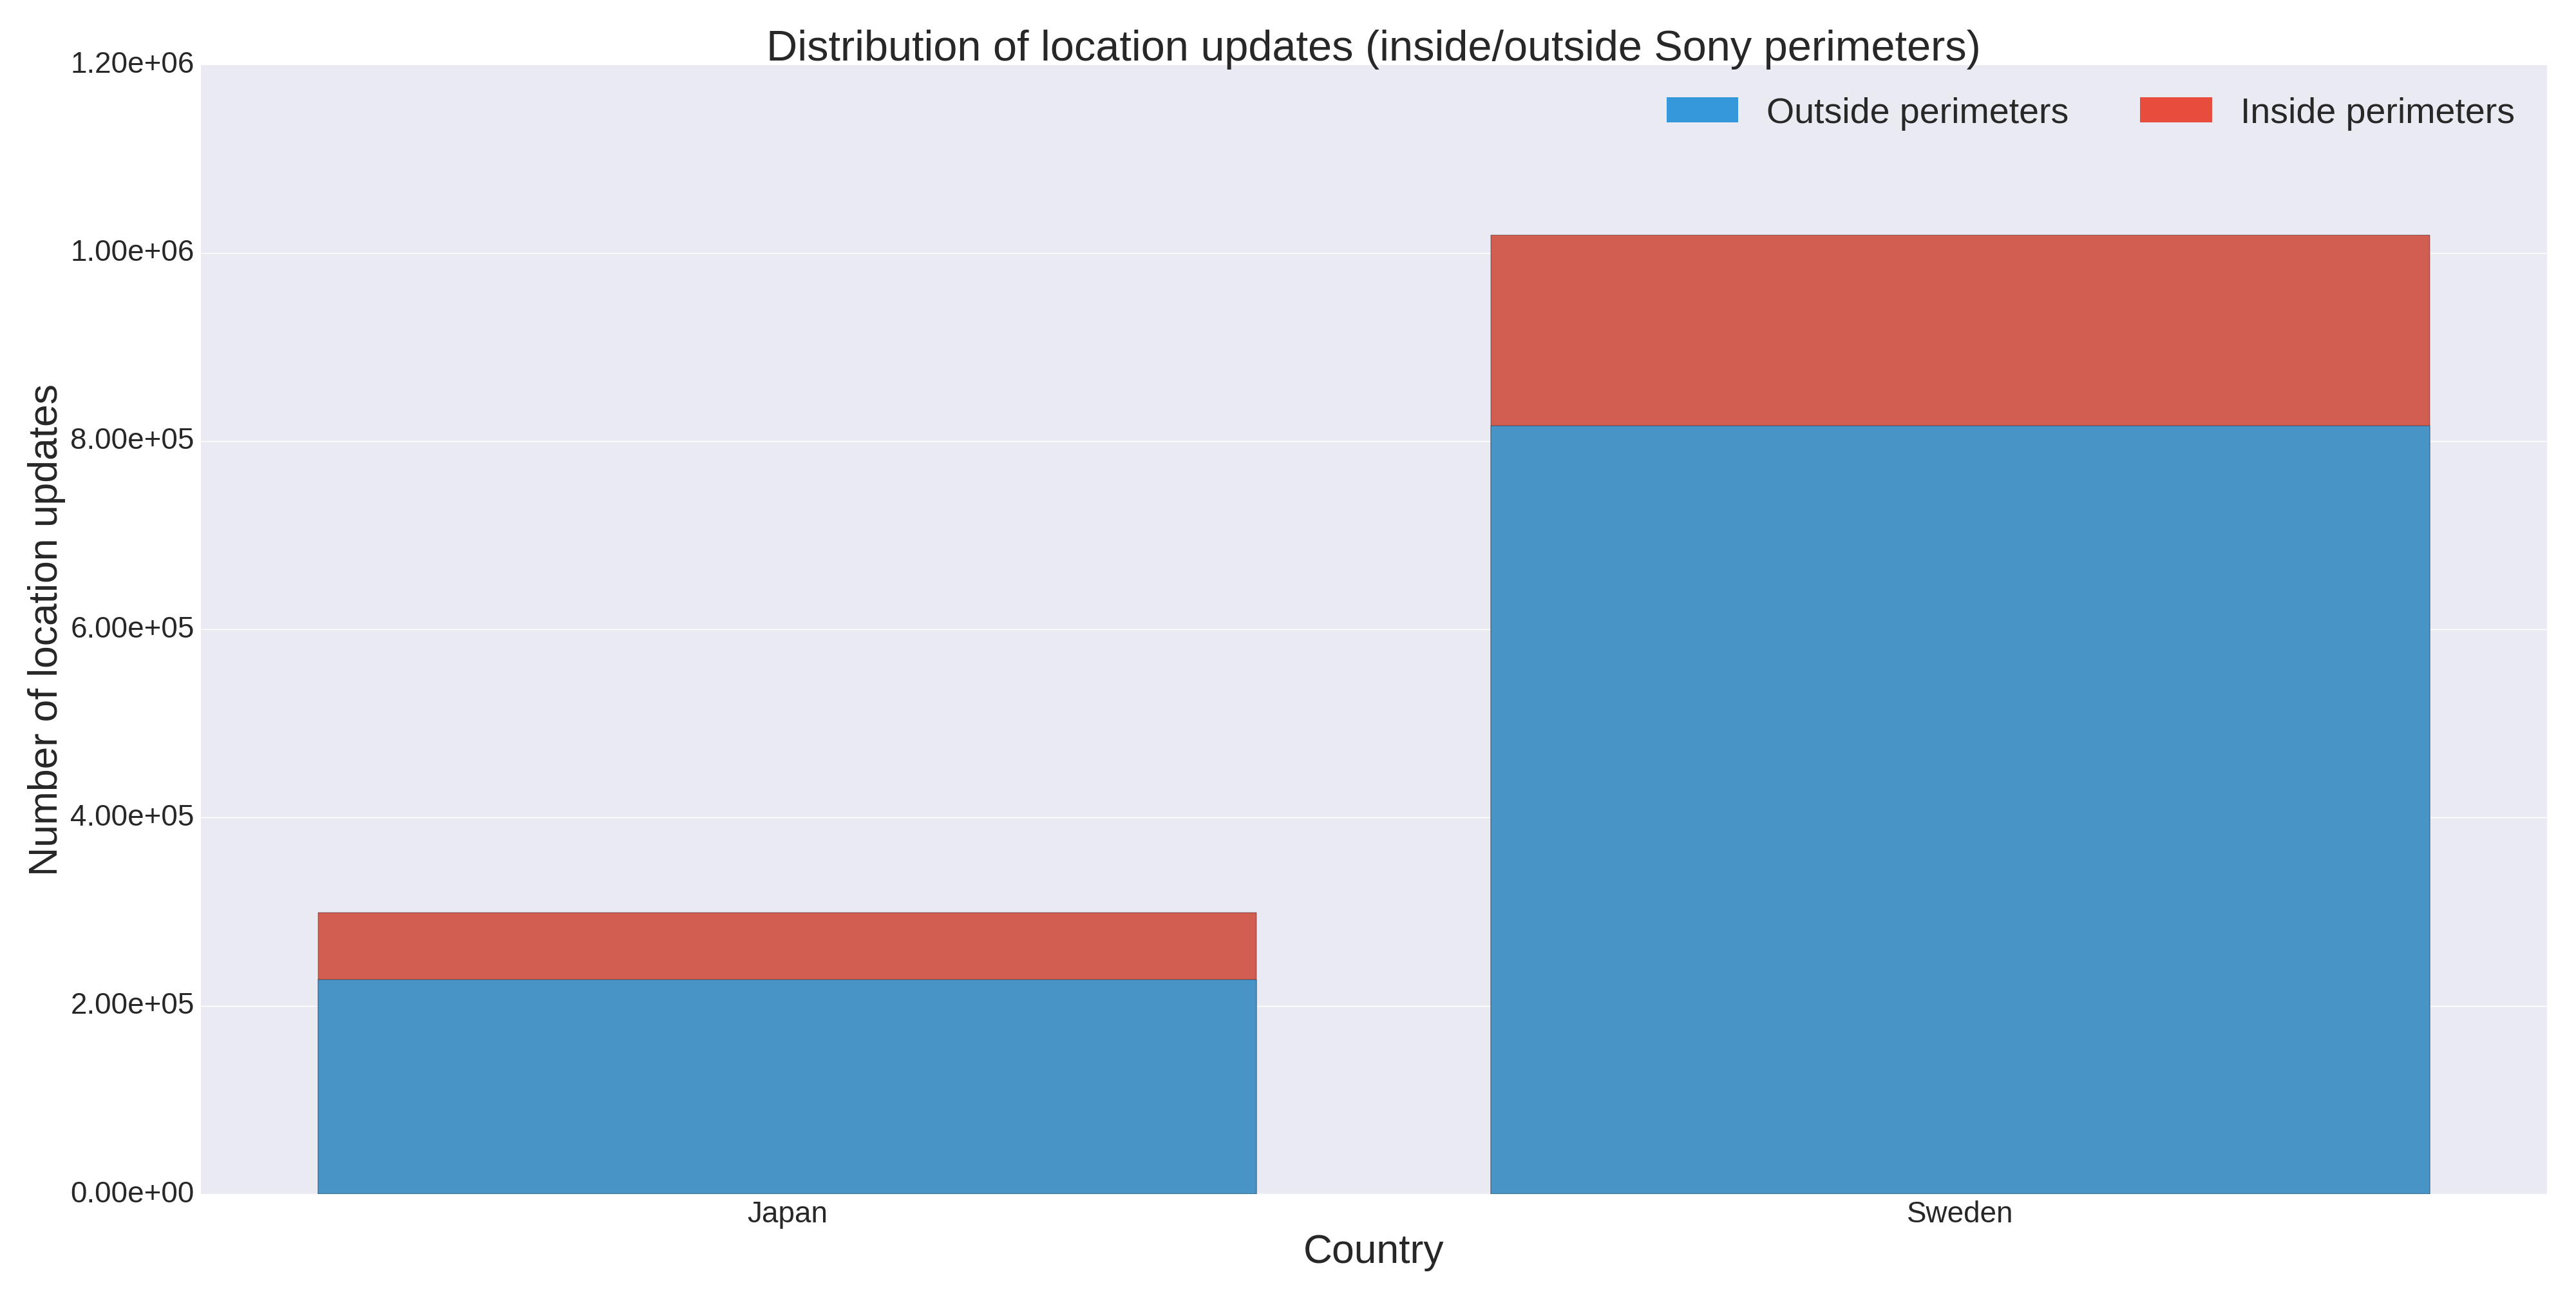
\includegraphics[scale=0.16]{stack_bar_loc_updates}
    \caption{Shows how many of the updates that is outside/inside Sony perimeters}
    \label{fig:hq_stack_bar}
\end{figure}

Figure \ref{fig:hq_stack_bar} viser hvordan opdateringerne fordeler sig mht. om de er forgået på et samlingssted eller ej. Vi ser at i begge landes tilfælde, er der en beskeden del der er indenfor samlingsstederne. For henholdsvis Japan og Sverige, svarer denne del til 23.89\% og 19.86\%. 
Dette tegner godt for projektet, at der er så stor del af opateringerne der ligger udenfor samlingstederne. 

Vi vil gerne se hvordan lokations opdateringerne for de to lande, er fordelt på brugerne. Til dette har vi quantilerne for de to lande, som se i Tabel \ref{tab:stat_loc_updates} 

\begin{table}[htbp]
        \centering
        \small
        \setlength\tabcolsep{2pt}
        \begin{tabular}{|c|c|c|c|c|c|c|c|c|c|c|}
            \hline
                         & Japan      &   Sweden      \\[-1pt]
            \hline
                 Min     &    1       &   1           \\
            \hline
                 Q1      &  26        &   68      \\
            \hline
                 Median  & 233     &   840      \\
            \hline
                 Mean    &  851.49   &  1,735.38     \\
            \hline
                 Q3      & 994.5    &   2,642     \\
            \hline
                 Max     &  9,320 &  14,759     \\
            \hline
                 IQR     &  968.5   &   2,574     \\
            \hline
            
        \end{tabular}
        \caption{Quantiles and mean over location updates for Japan and Sweden} %add this between 'caption' and '{...' for new text in listing of tables: [New caption text only for listing of tables]
        \label{tab:stat_loc_updates}
\end{table}


Hvis vi kigger på landenes quantiler, kan vi se at 25\% quantilen (Q1) er meget lav hos begge lande. Q1 vise med andre ord, at 25\% af brugerne i Japan og Sverige har henholdsvis maksimalt 22 og 71 opdateringer, henover alle tre måneder. Dette er ikke et godt tegn at så mange brugere har så få opdateringer. 75\% quantilen (Q3) er en del højere i Sverige end i Japan, hvilket viser der er 75\% af brugerne der har maksimal 1,063.25 og 2,848.25 lokations opdateringer i henholdsvis Japan og Sverige. Dette ser igen bedre ud i Sverige, hvis brugere har flere opdateringer end Japan. \\ 

Begge lande har en lille procent brugere, som står får utroligt mange opdateringer. I Sverige er der 25\% brugere som har mellem 2,848.25 og 15,447 opdateringer og i Japan har de mellem 1,063.25 og 10,316 opdateringer. Dette er ligesom med Q1 et dårligt tegn. 
Median og mean er meget større i Sverige end Japan. Dette tyder på at der er flere brugere med flere lokations opdateringer i Sverige end i Japan. \\


Den ovenstående tendens, vil vi gerne vise mere tydeligt, hvorfor vi har plottet den Cumulative Distribution Function (CDF) for de to lande. 
\begin{figure}[H]
    \hspace*{-1.0cm}
    \centering
    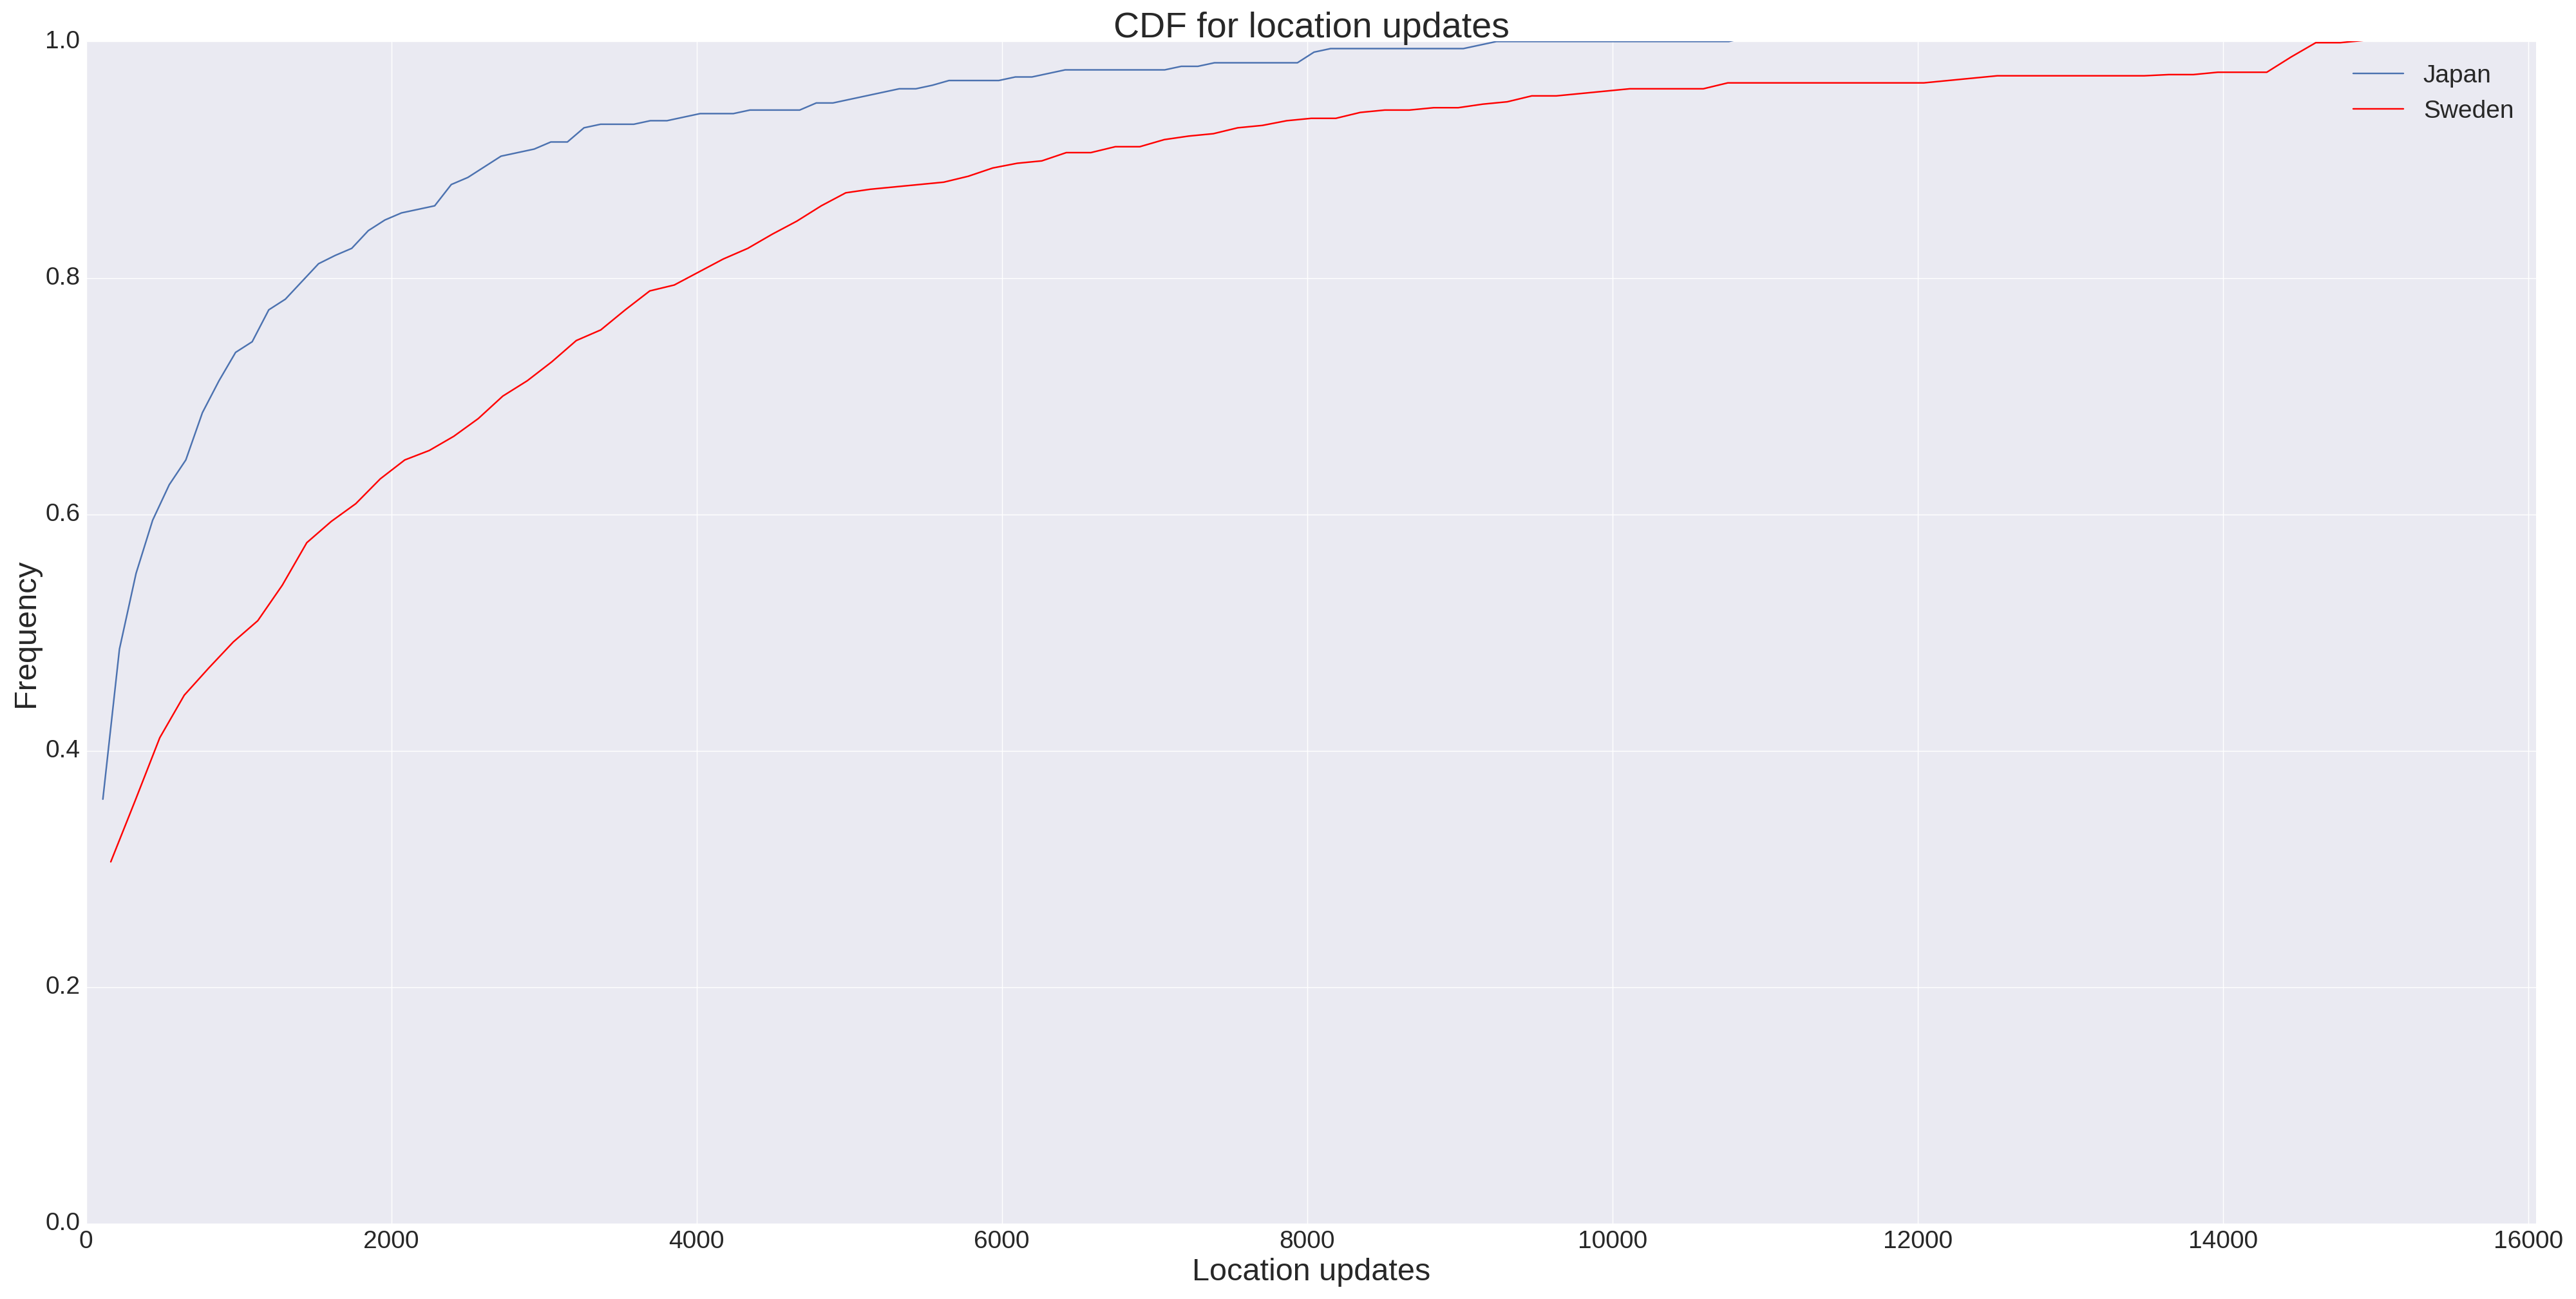
\includegraphics[scale=0.14]{cdf_location_updates_swe_jap}
    \caption{Cumulative Distribution Function (CDF) over location updates for Japan and Sweden henover periodens tre måneder}
    \label{fig:country_cdf}
\end{figure}

Plottet viser, at der både i Japan og Sverige er en stor del af brugerne, som har meget få lokations opdateringer set henover hele perioden. Det kan ses, at Japan får hurtigt flere brugere med få opdateringer, end Sverige. 
Da opdateringerne kommer hver gang brugeren skifter lokation, betyder dette, at mange af brugerene er meget stillestående eller også har de slukket mobilen. Her kan stillestående også menes, at brugeren har glemt sin telefon derhjemme. Vi kan se forskel i dataen på, om de har slukket mobilen eller er stillestående, men ikke om de er stillestående eller har glemt mobilen. Vi kan se den førstnævnte forskel ved, at der simpelthen mangler data i et tidsrum, hvor hvis brugeren er stillstående er intervallet mellem \texttt{start\_time} og \texttt{end\_time} markant. 

Vi vil gerne se om der er et mønster i hvornår opdateringerne kommer, da vi derfra muligvis kan udpege bedre eller dårligere sub-perioder som vi kan tage stilling til. Derfor har vi lavet nogle heat maps. 
De første heat maps viser hvordan opdateringerne er fordelt over et døgn. Dette er lavet, ved at aggregerer over tidsrummet i det pågældende døgn. Det der bliver aggregeret er, om en brugere har haft mindst én opdatering, i det tidsrum på døgnet (repræsenteret med 0 eller 1), uanset hvilken dag det er.

Figure \ref{fig:agg_heatmap_jap} viser hvordan opdateringerne for hver user (y-aksen), fordeler sig over tidsrummet på en dag, målt over alle tre måneder. Det ses at skalaen går til ca. 70, hvilket betyder at brugeren med flest aggregerede opdateringer i et time-slot (på en time), har ca. 70 opdateringer henover alle tre måneder. Brugerne er sorteret på baggrund af deres samlede aggregerede værdier, men den største nederst på y-aksen. 

Man ser tydeligt, at der er en periode mellem kl. 02:00 og kl. 06:00 hvor de fleste brugere ikke har nogle updates, dette kunne tyde på at de enten slukker eller på anden måde lukker for kommunikationen med omverdenen i det givne tidsrum. Herefter fra kl. 06:00 til 00:00 er der regelmæssig opdateringer, hvorefter det stilner af til kl. 02:00. Hvis vi sammenligner dette med Figure \ref{fig:cumu_loc_time_jap_swe} kan vi se det stemmer meget godt overens. Figure \ref{fig:cumu_loc_time_jap_swe} viser den cumulative location updates henover et døgn i både Japan og Sverige. Her ser vi samme udvikling for Japan som heat mappet indikerer, som beskrevet ovenfor. 

Det ovenstående gælder også for Sverige (Figure \ref{fig:agg_heatmap_swe}), som viser det samme som Japan. Her slukker næsten alle brugere også deres mobiler mellem 02:00 og 06:00
Der er ikke andre time-slots som skilder sig ud, hverken i Japan eller Sverige. 

Da vi har sorteret brugerne kan vi nemt se, at der er en del brugere som ikke har nogle, eller meget få, opdateringer henover alle tre måneder. Disse bruge kunne vi se bort fra i vores forsøg, da de alligevel ikke bidrager med noget. 

\begin{figure}[H]
    \hspace*{-0.8cm}
    \centering
    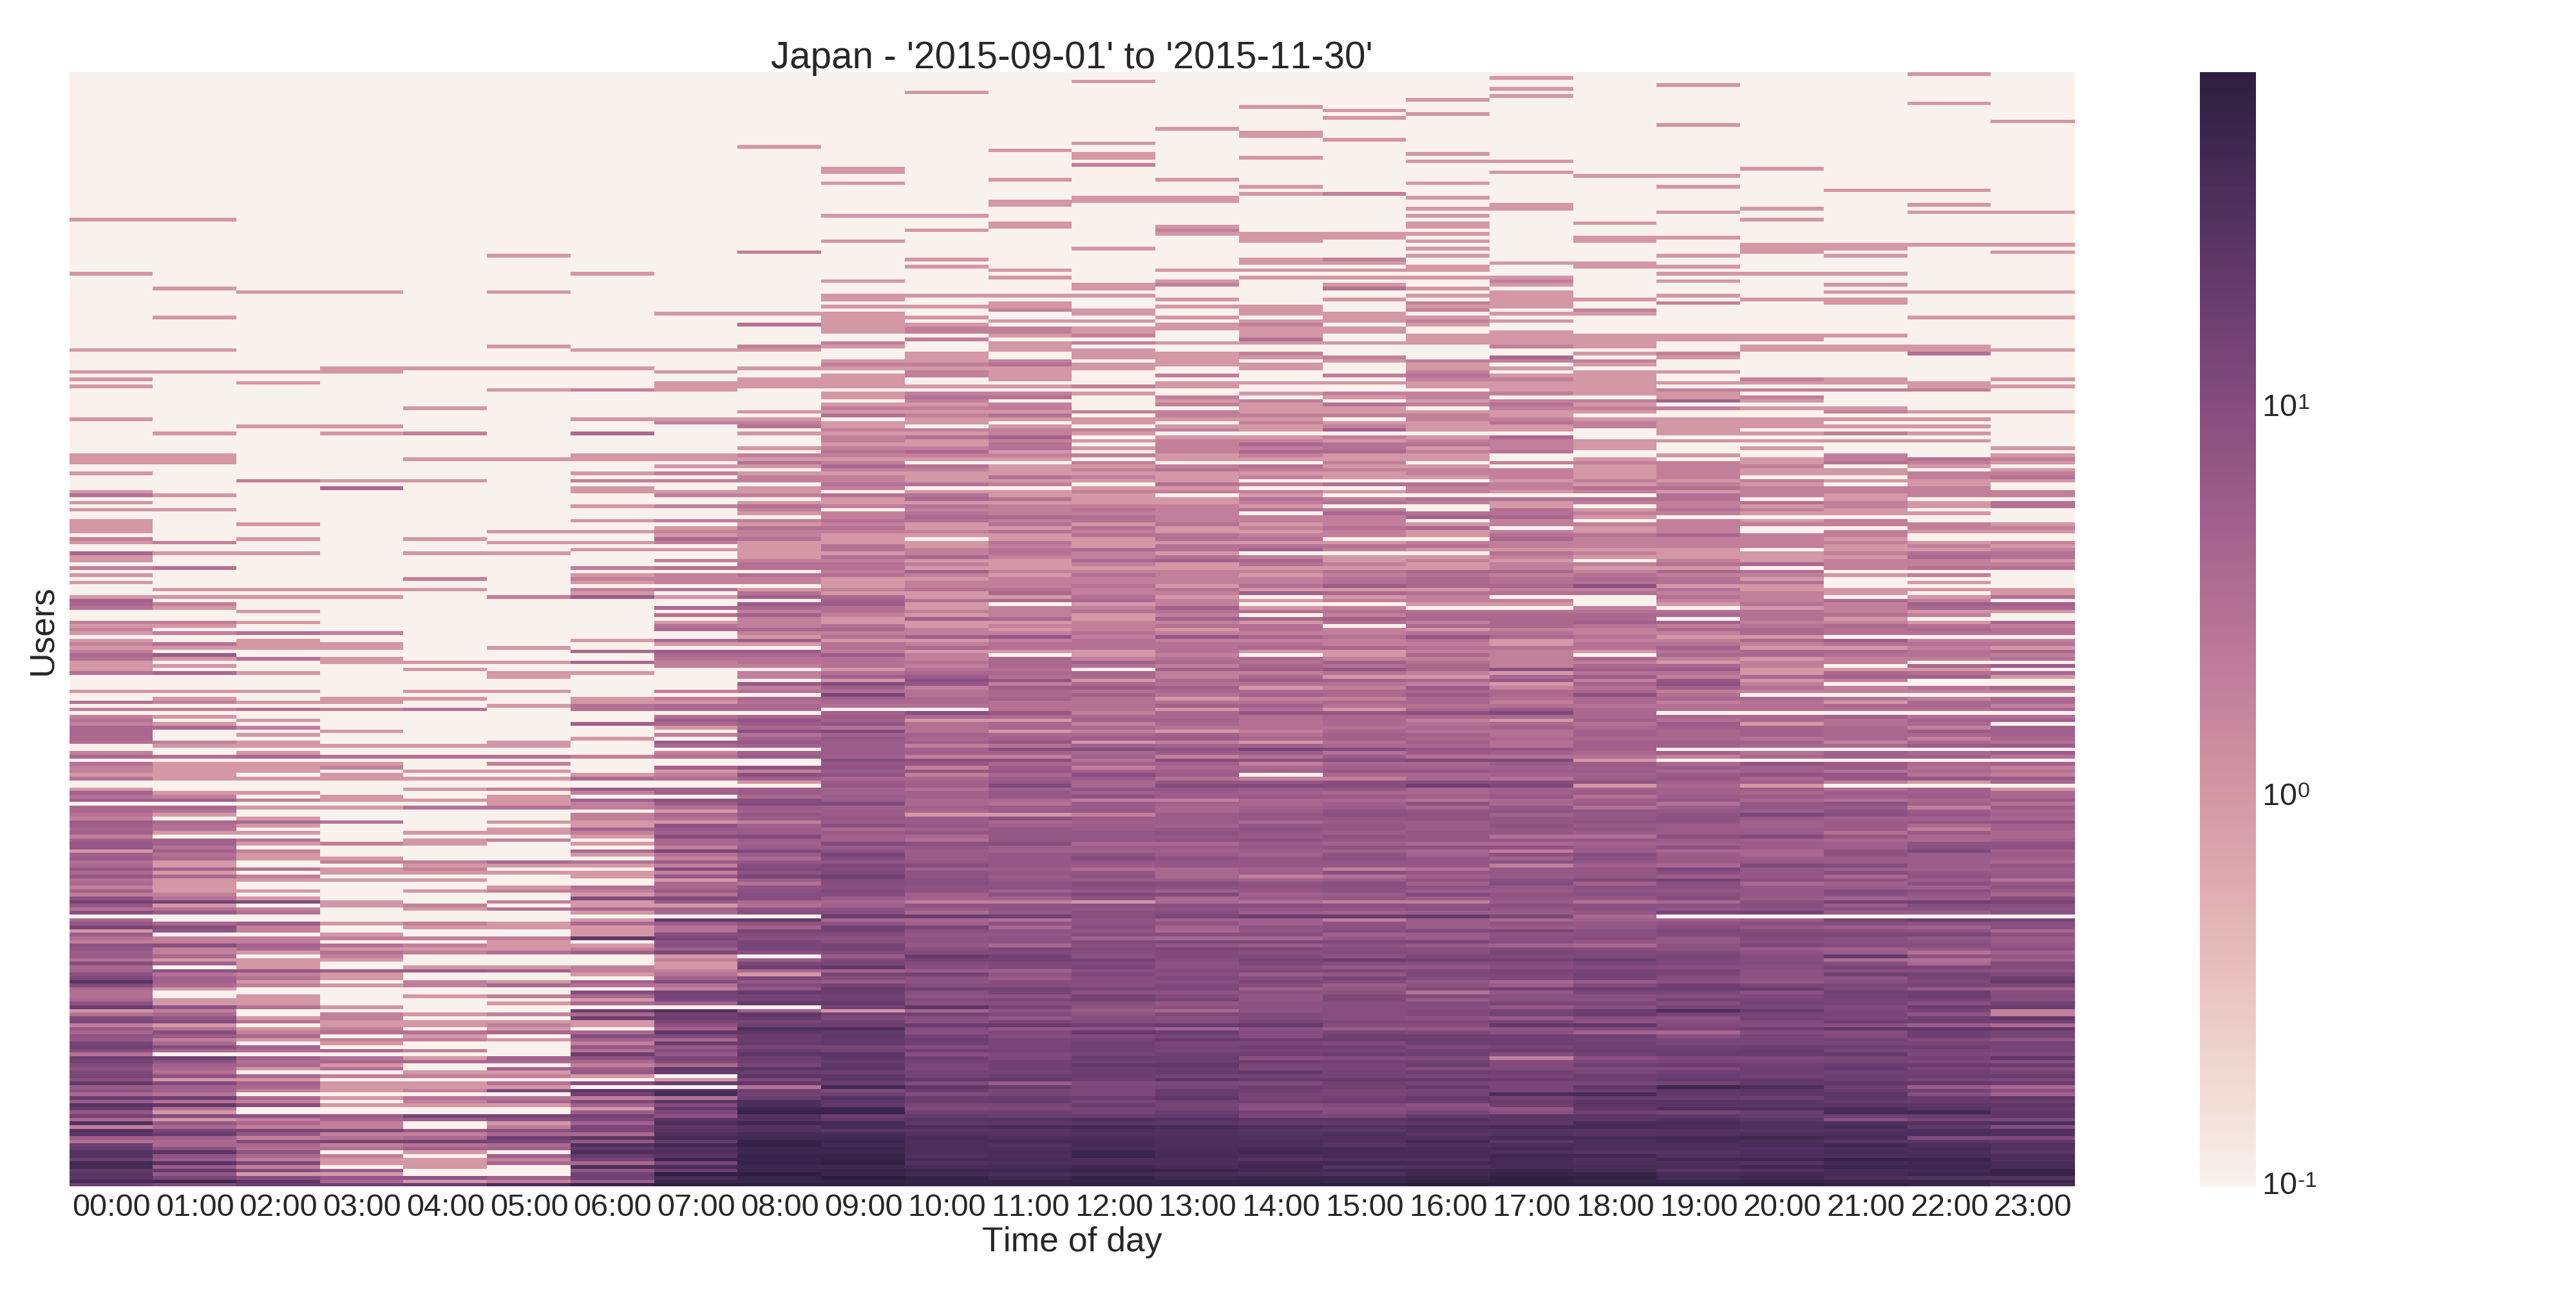
\includegraphics[scale=0.15]{aggregated_updates_over_time_japan}
    \caption{Heat map for location updates over the 3 month period in Japan, aggregated over a day with 60 minutes of binsize. Users are sorted by total number of location. Largest is at the bottom}
    \label{fig:agg_heatmap_jap}
\end{figure}
\begin{figure}[H]
    \hspace*{-0.8cm}
    \centering
    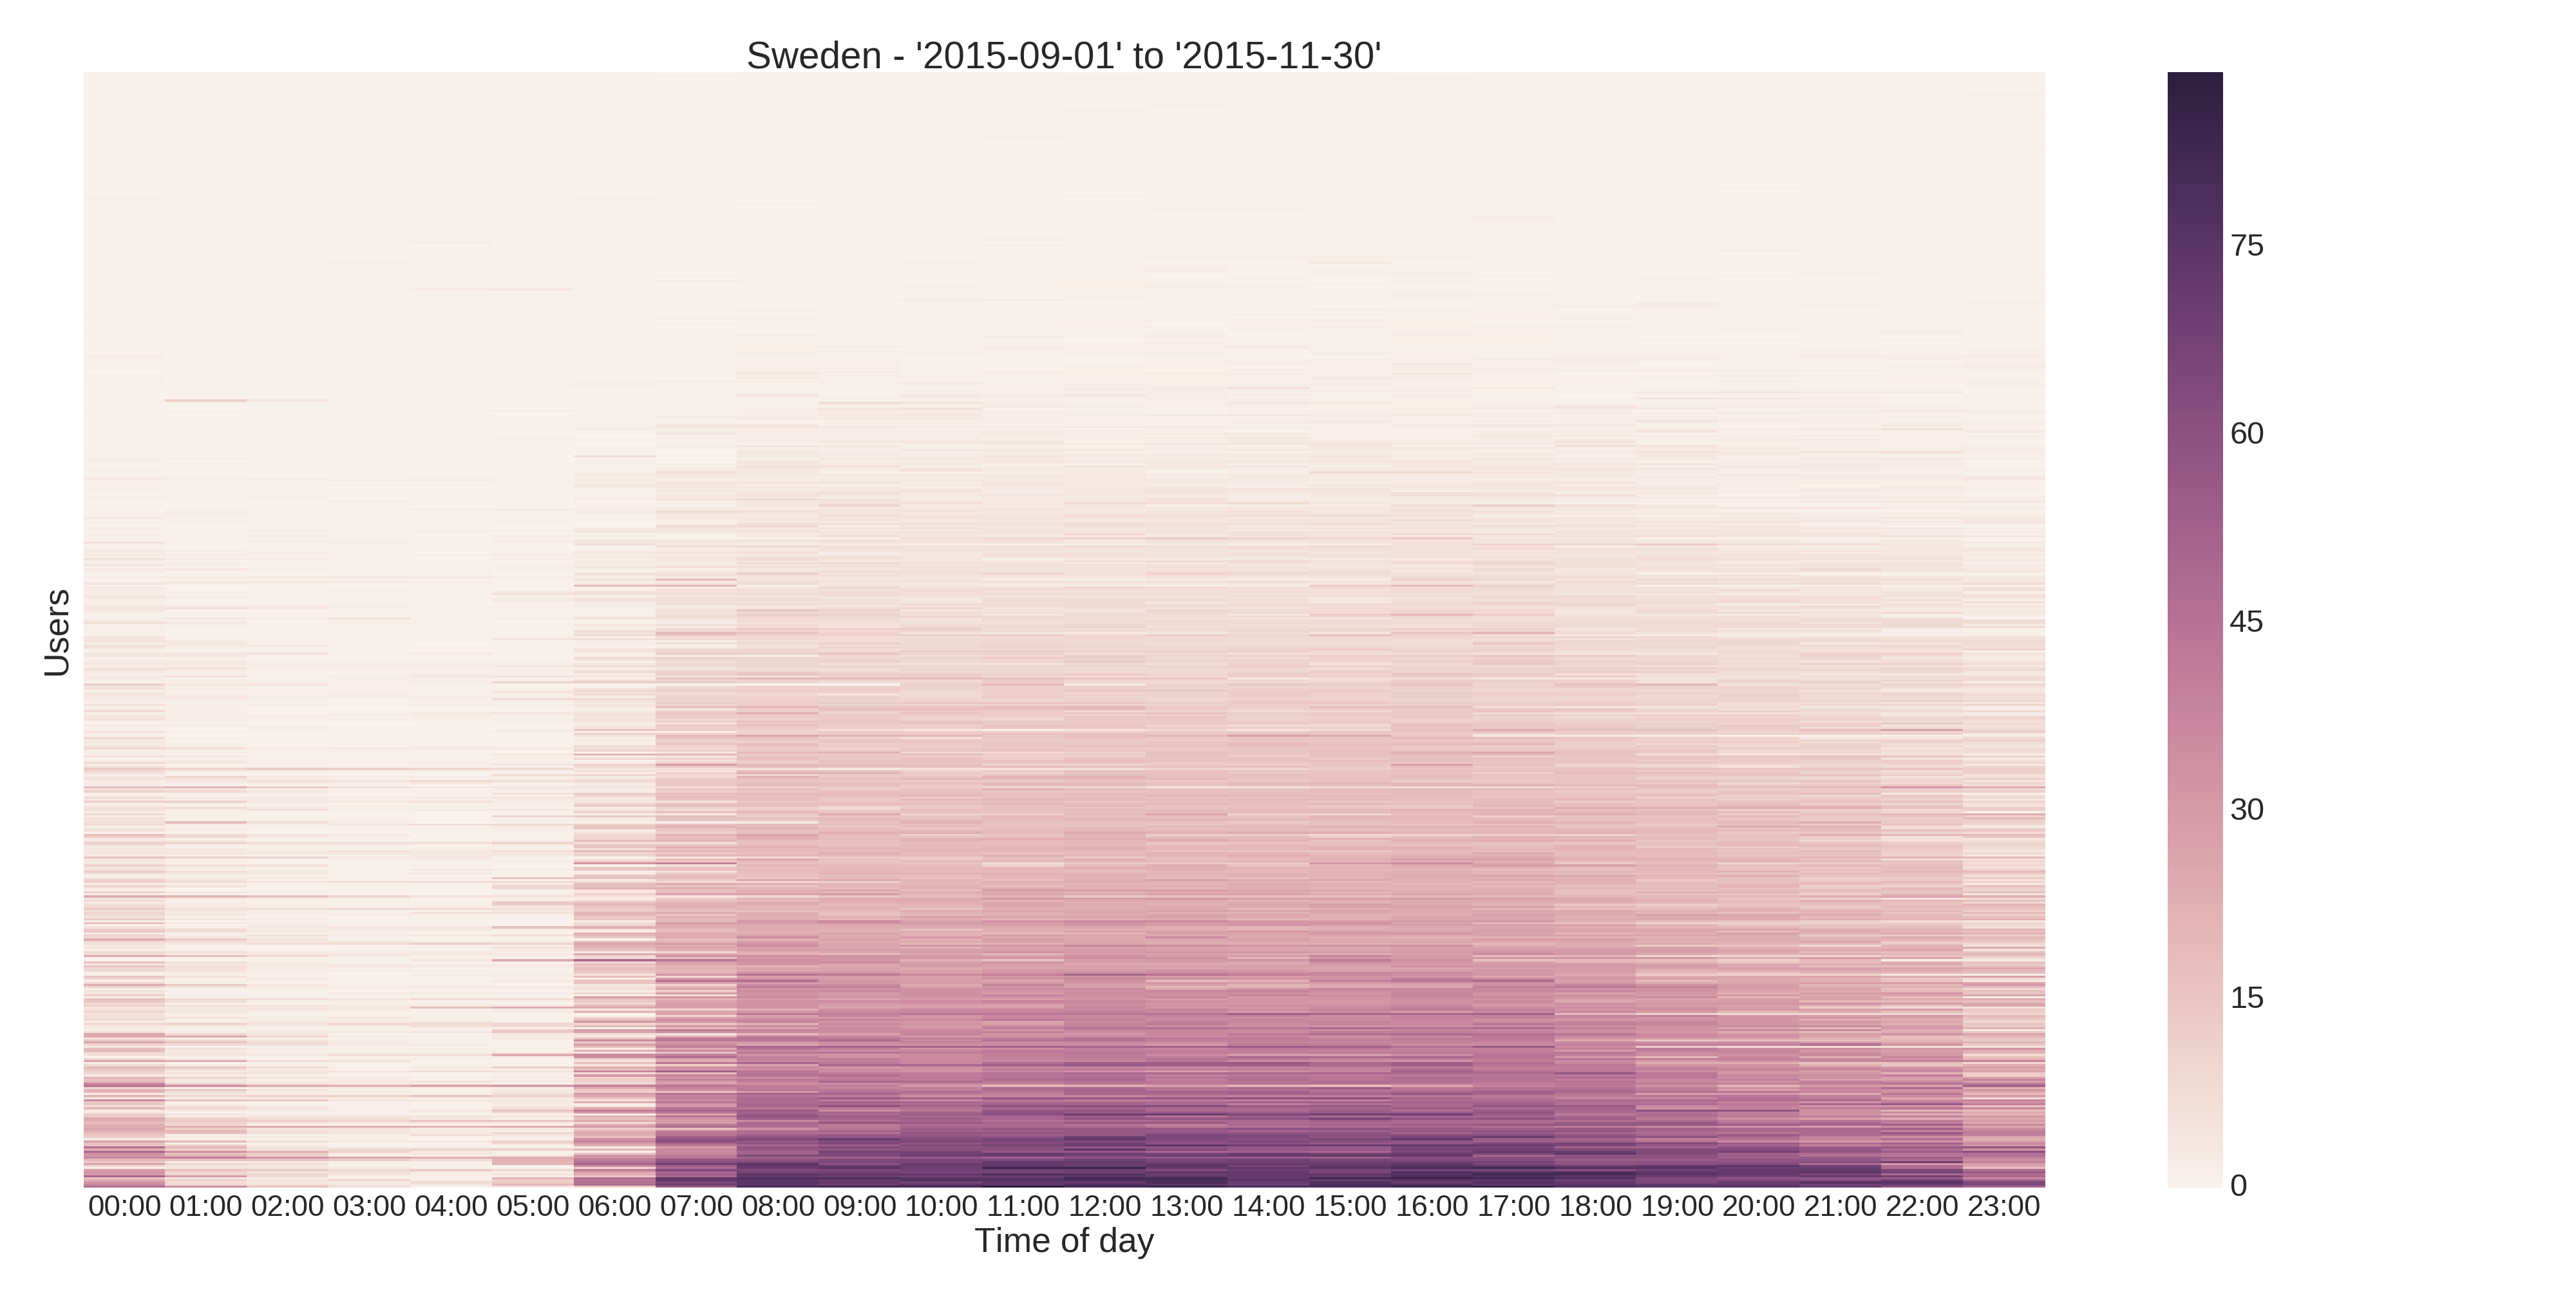
\includegraphics[scale=0.15]{aggregated_updates_over_time_sweden}
    \caption{Heat map for location updates over the 3 month period in Sweden, aggregated over a day with 60 minutes of binsize. Users are sorted by total number of location. Largest is at the bottom}
    \label{fig:agg_heatmap_swe}
\end{figure}

\begin{figure}[H]
    \hspace*{-1.8cm}
    \centering
    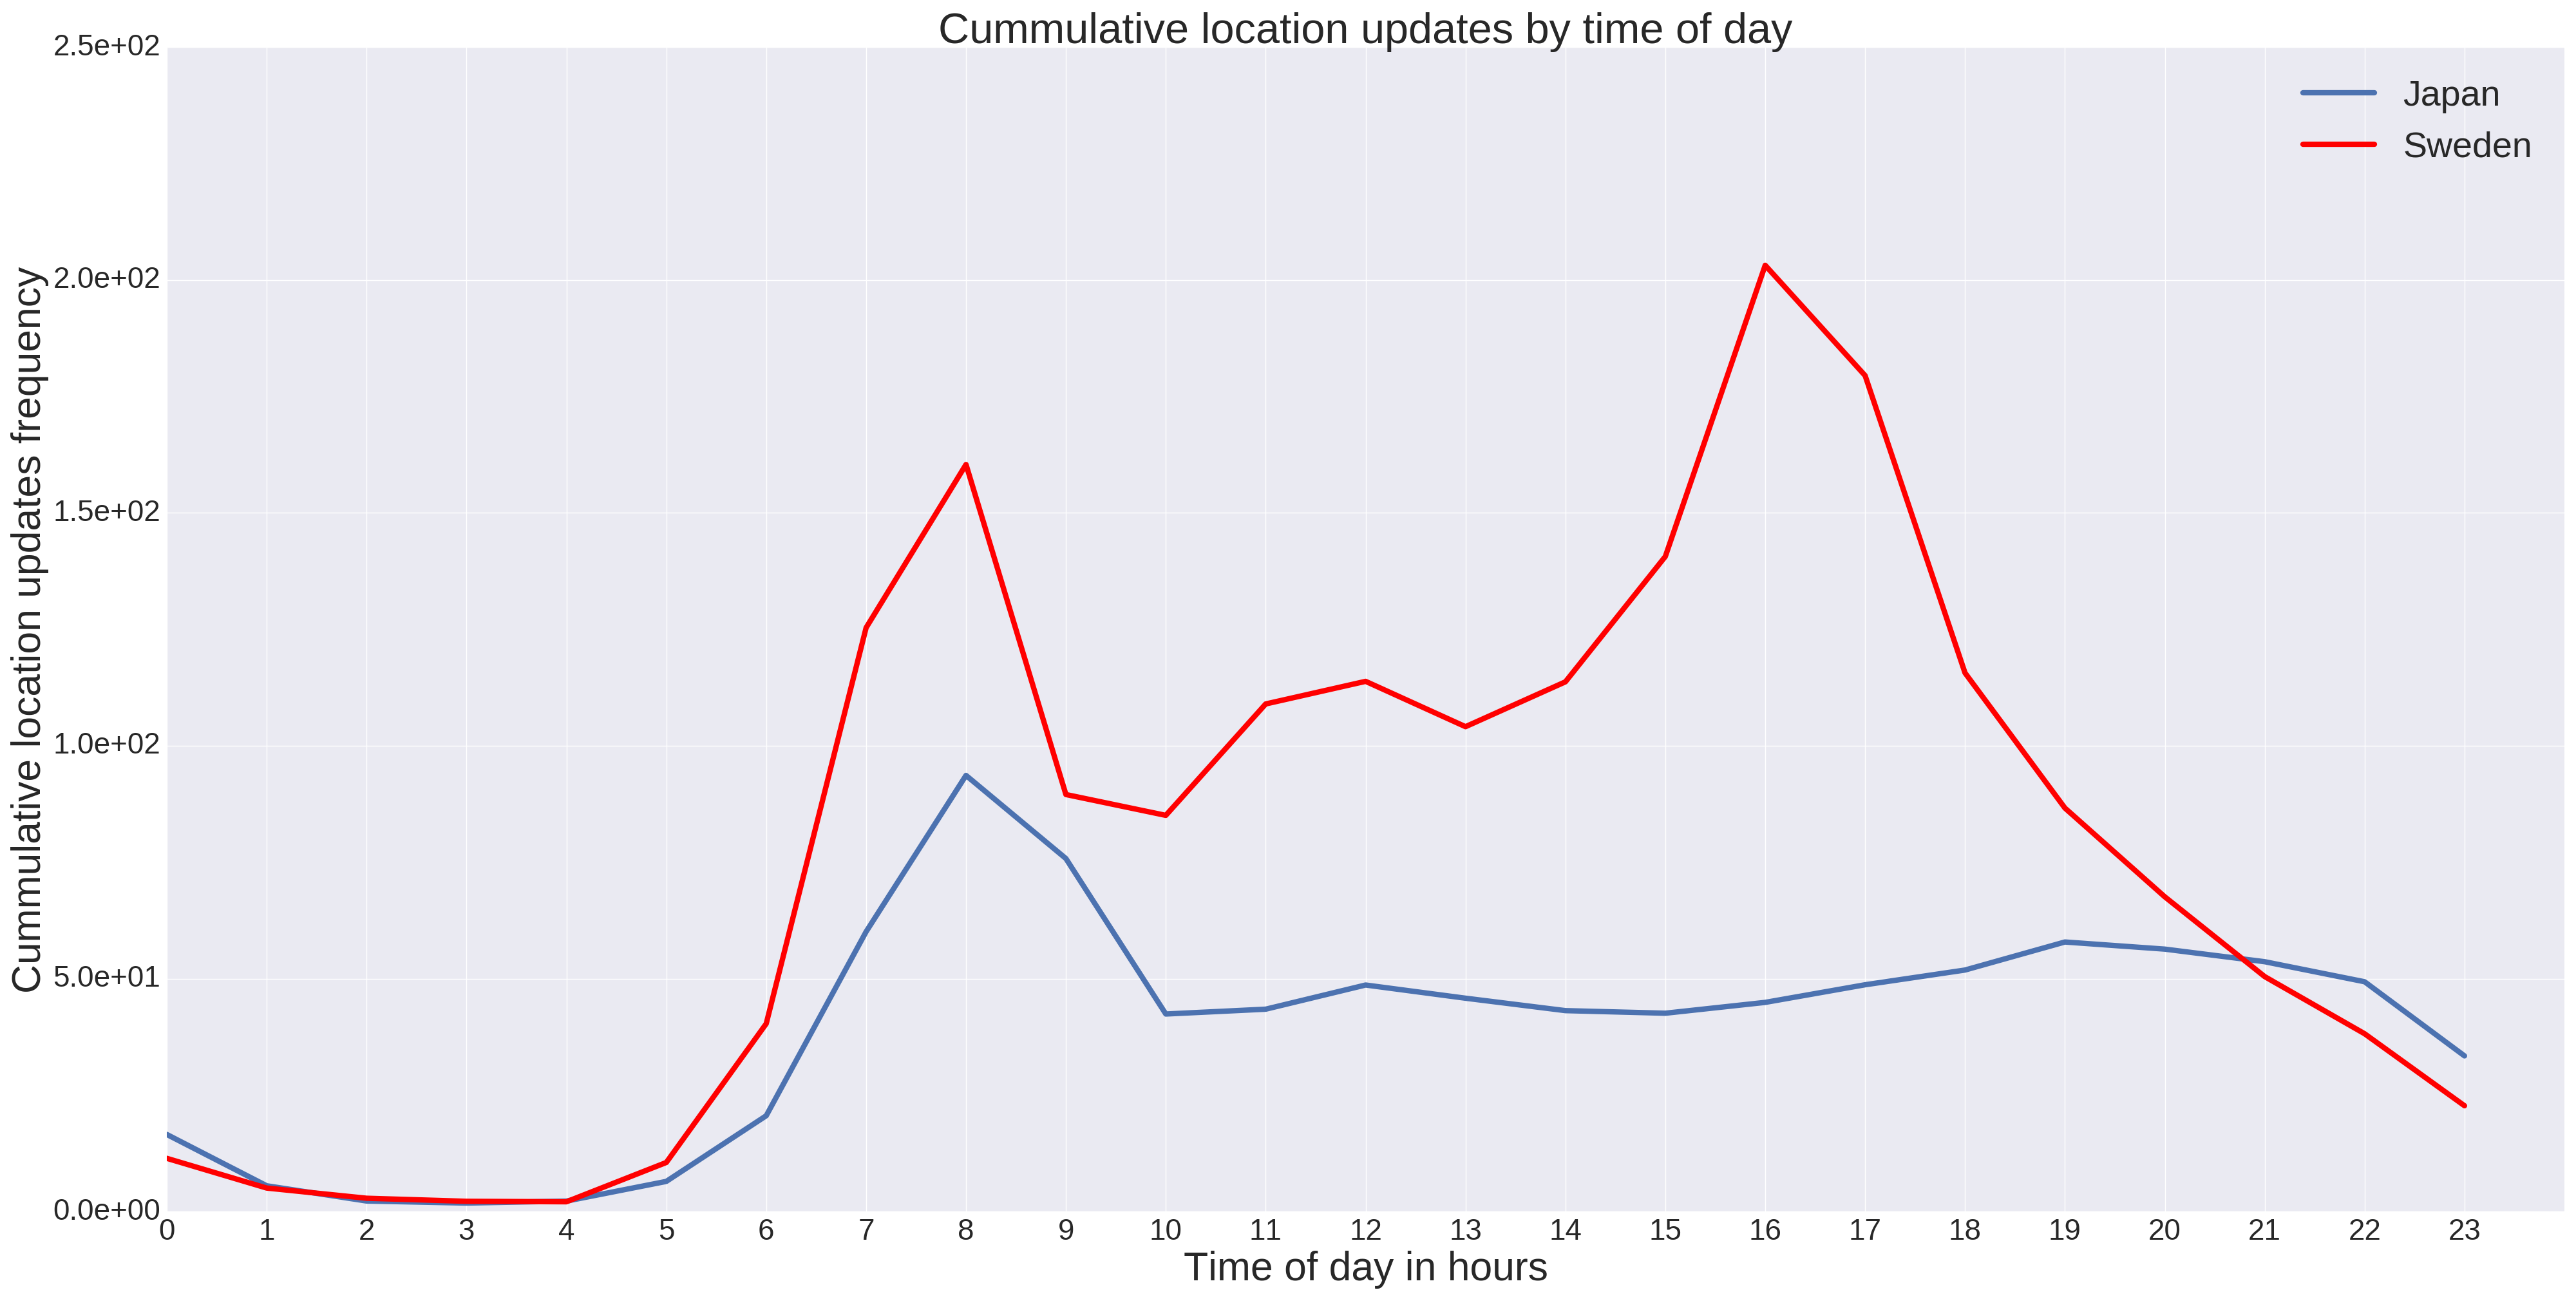
\includegraphics[scale=0.15]{cumulative_updates_overTime_swe_jap}
    \caption{Shows when the cumulative location updates occuring over a day. The value of the updates are normalized}
    \label{fig:cumu_loc_time_jap_swe}
\end{figure}

Hvis vi udelukkende kigger på Figure \ref{fig:cumu_loc_time_jap_swe}, kan vi se at det topper i begge lande omkring kl. 08:00 om morgenen. I Sverige topper det desuden også kl. 16:00, hvor det ikke gør det i Japan. Her er det neutral. \\
Toppen der finder sted kl. 08:00 om morgen, skyldes nok at brugerne er på vej til arbejde og derved får en masse updates. Tilsvarende kan den anden top (i Sverige), være der hvor brugerene er på vej hjem fra arbejde, hvor man derved også får en masse updates. Det bemærkes at Japan ikke har en tilsvarende stigning i locations updates ved eftermiddagen, men dog har en lille stigning ved 19:00 og højere værdier end Sverige fra 21:00-23:00.\\

Begge disse scenarier tegner ikke godt for vores mål, da det giver sig selv at der skal være nogle data for at finde co-occurences. 
På baggrund af quantiles og CDF, kunne det tyde på at data fra Sverige vil være mere brugbart end Japan. 

Når vi nu ved, at største delen af brugerne i begge lande har få opdateringer, vil vi gerne vide hvodan disse opdateringer er fordelt henover perioden. Det er interssant for os at vide, om opdateringerne er ligeligt fordelt på dagene eller om de klumber sig sammen. Det er interessant, da det kan gøre en forskel med hvad vi bruger til vores modeller. 

Vi har valgt at visualisere dette, ved brug af Heatmaps. 

\newpage


\begin{figure}[H]
    \hspace*{-1.5cm}
    \centering
    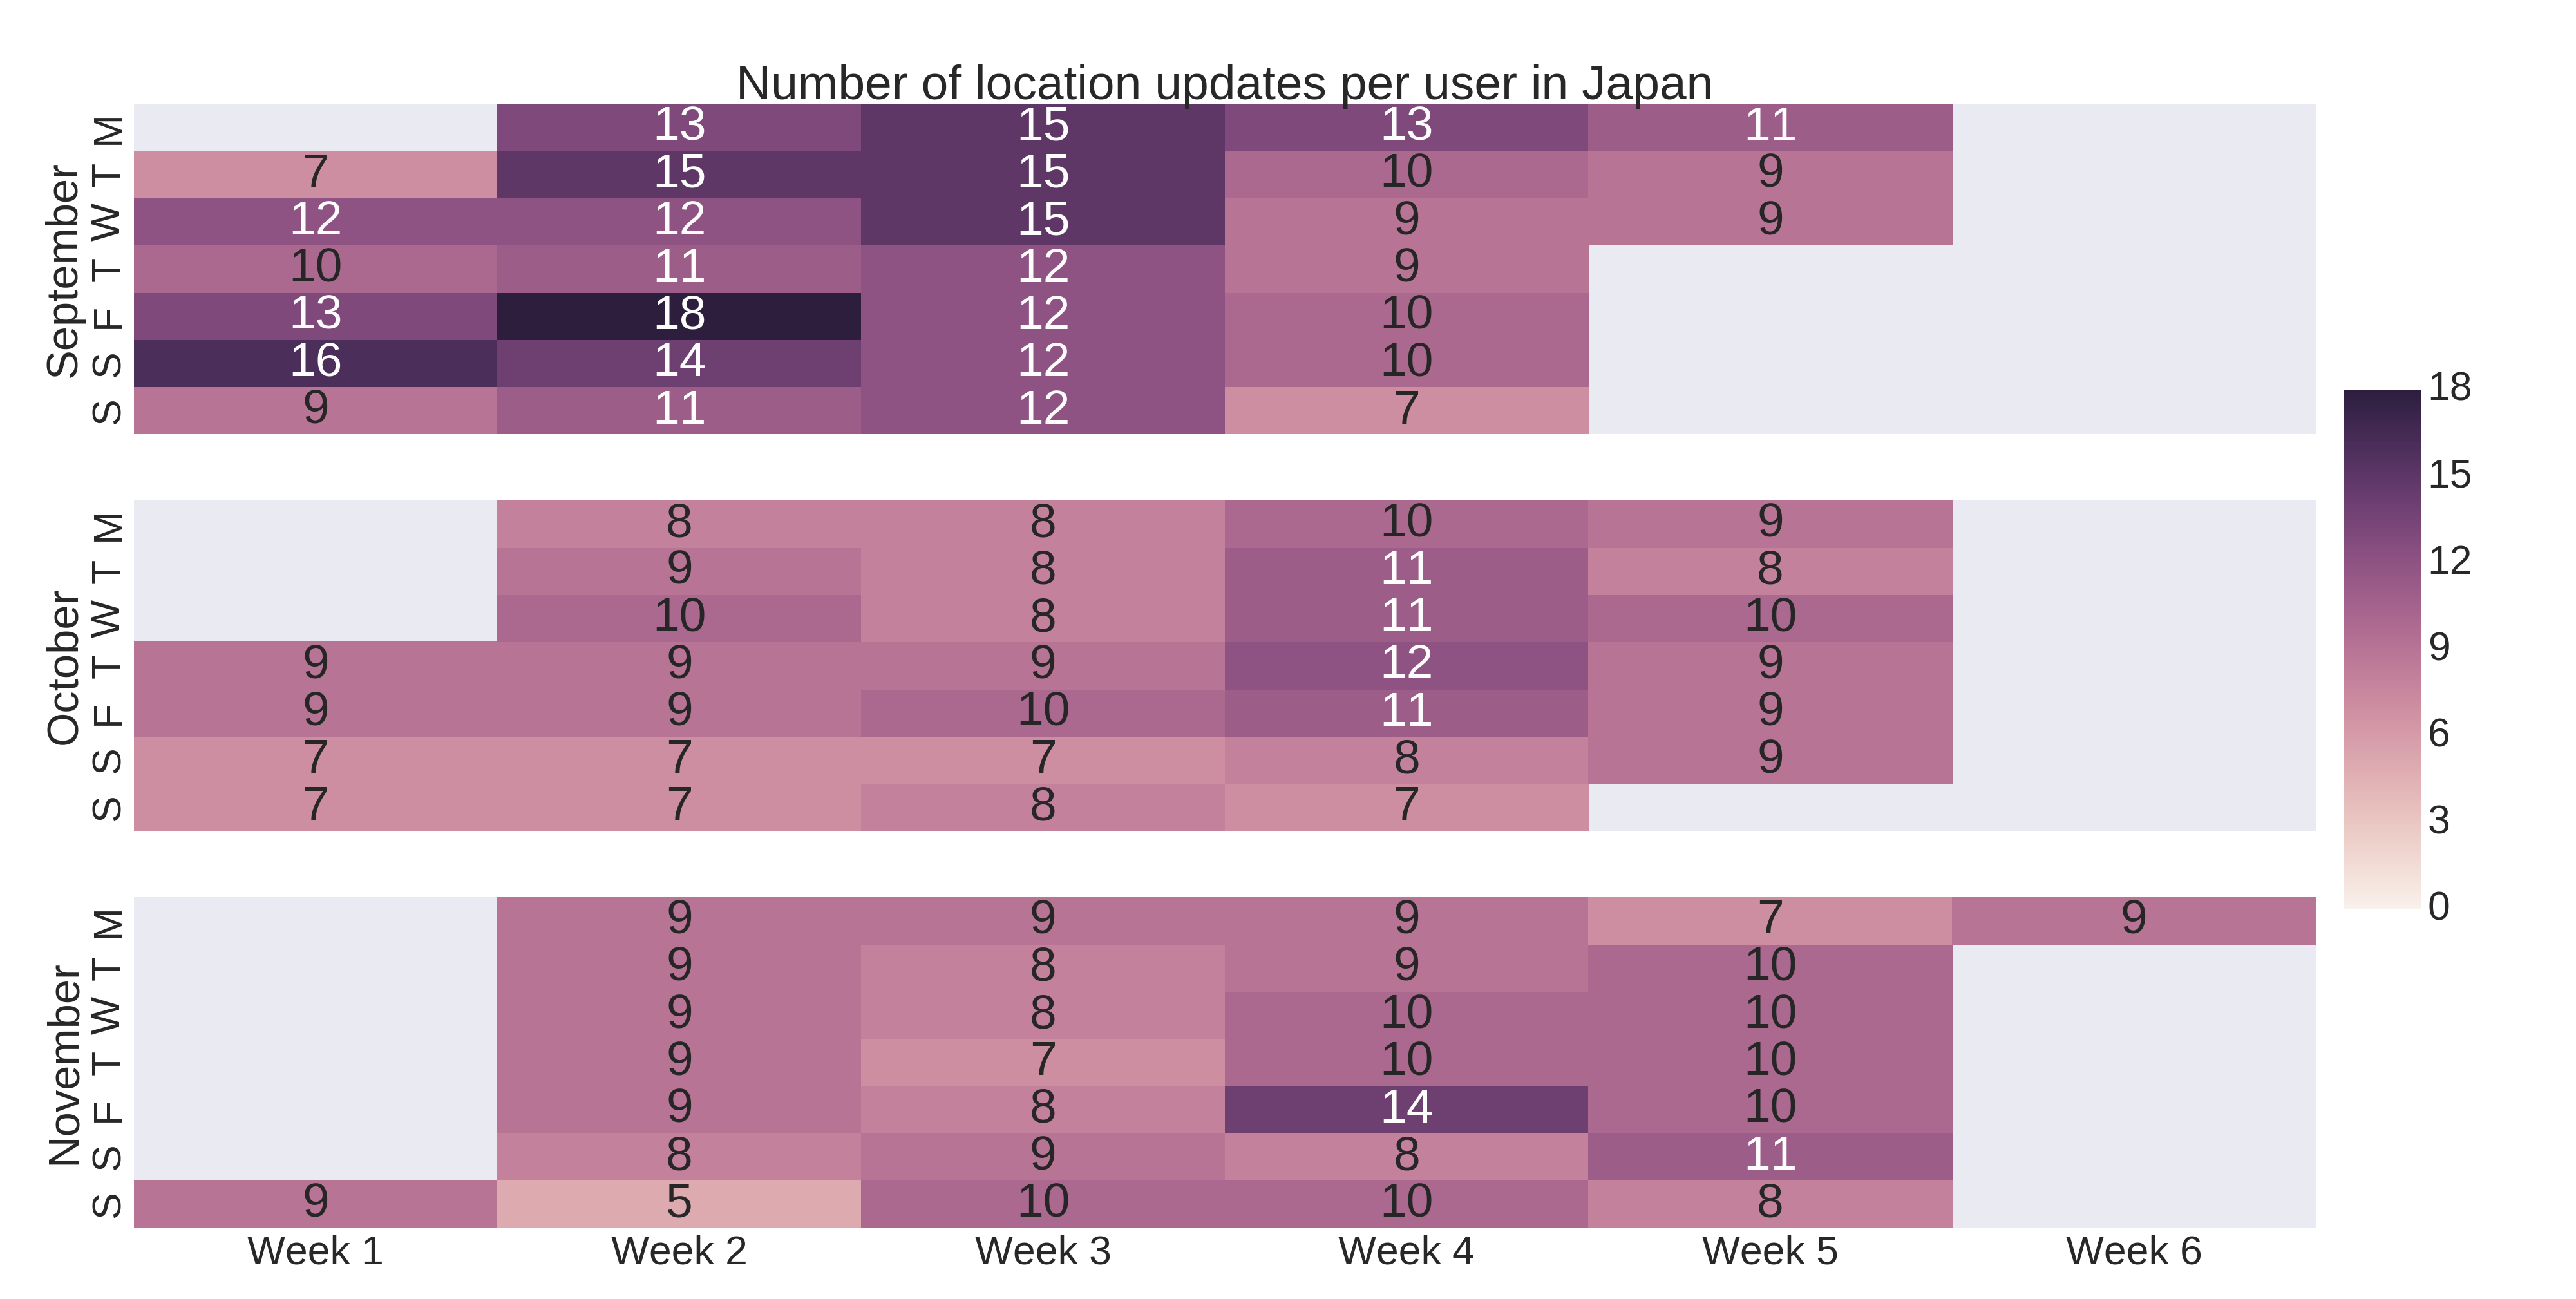
\includegraphics[scale=0.15]{heatmap_location_updates_japan}
    \caption{Heat map for mean location updates over the 3 month period in Japan}
    \label{fig:heatmap_jap}
\end{figure}
\begin{figure}[H]
    \hspace*{-1.5cm}
    \centering
    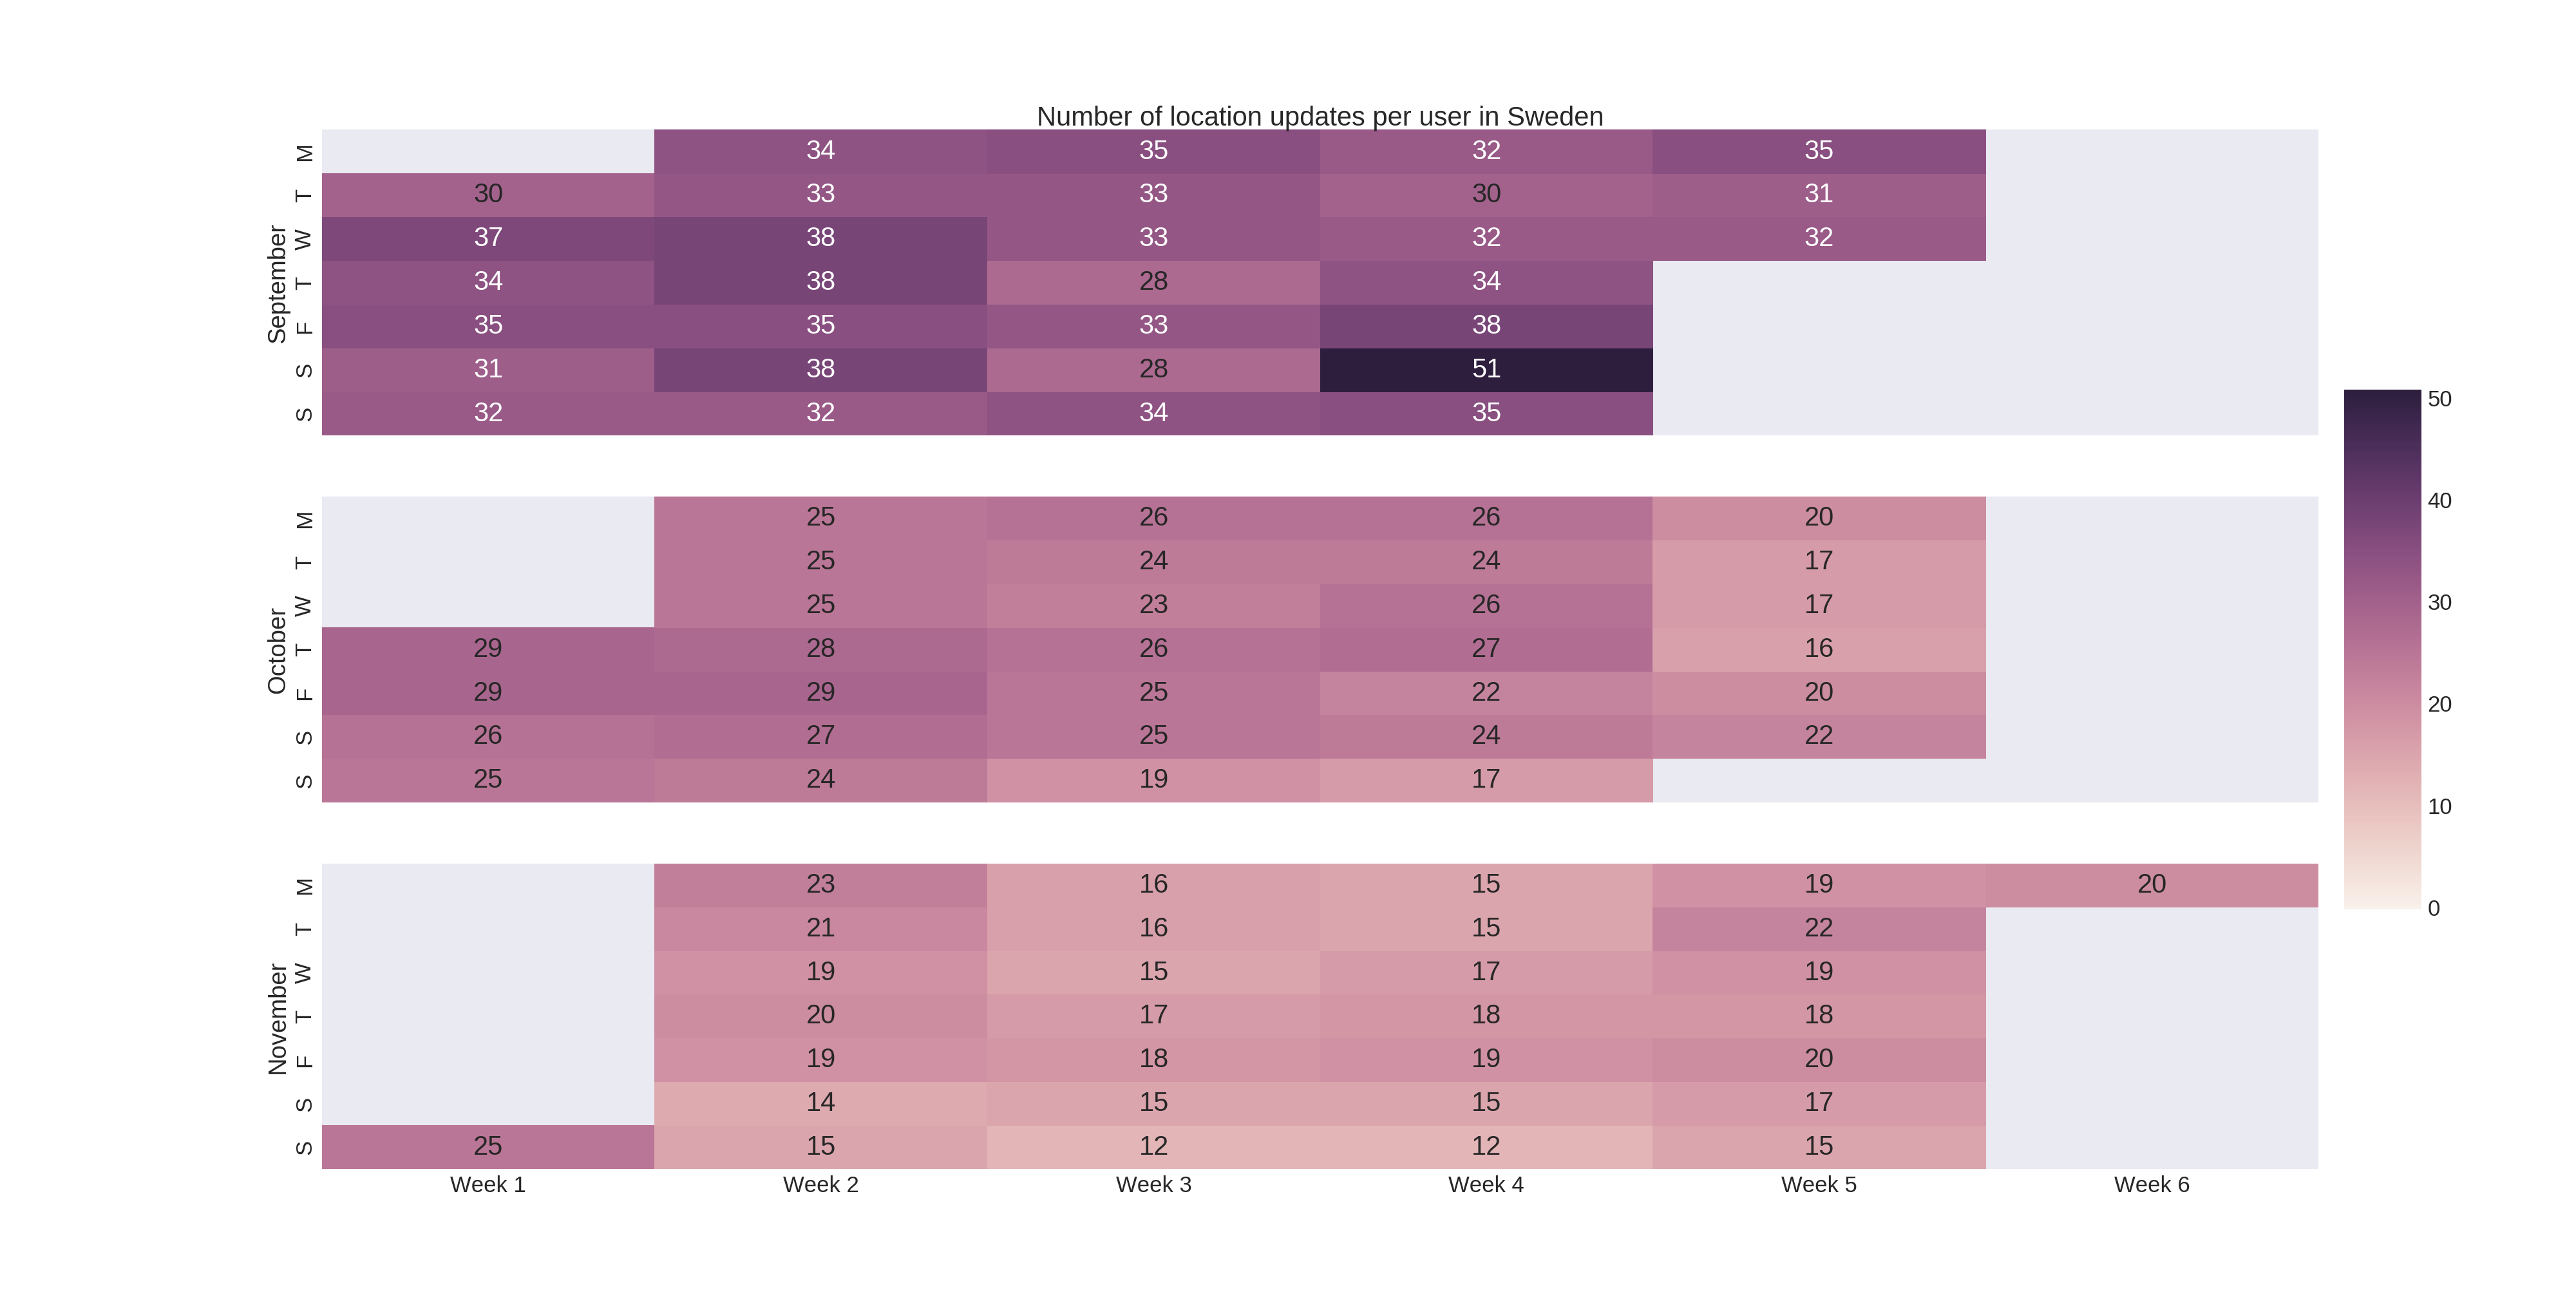
\includegraphics[scale=0.15]{heatmap_location_updates_sweden}
    \caption{Heat map for mean location updates over the 3 month period in Sweden}
    \label{fig:heatmap_swe}
\end{figure}


 Figure \ref{fig:heatmap_jap} viser hvordan lokations opdateringerne per bruger (afrundet til heltal) i Japan er fordelt over hver dag i hver af de tre måneder. Figure \ref{fig:heatmap_swe} viser det samme, bare for Sverige. 
 Vi kan f.eks. se, at der i Japan er gennemsnitligt 18 opdateringer per bruger om fredagen i uge 2 i september, hvor der samme dag i Sverige er 29 opdateringer. 

 Vi kan se at for både Japan og Sverige gælder, at der generelt er mere aktivitet i september, end i de andre måneder. Dette underbygger tendensen fra Figure \ref{fig:mean_loc_updates_sep-nov}, hvor vi kunne se en nedadgående tendens fra september til november. I Japan er october og november på nogenlunde samme niveau, hvor man i Sverige tyderligere kan se en ydeligere reducering af antal opdateringer. 

 
\newpage

\begin{figure}[H]
    \hspace*{-1.5cm}
    \centering
    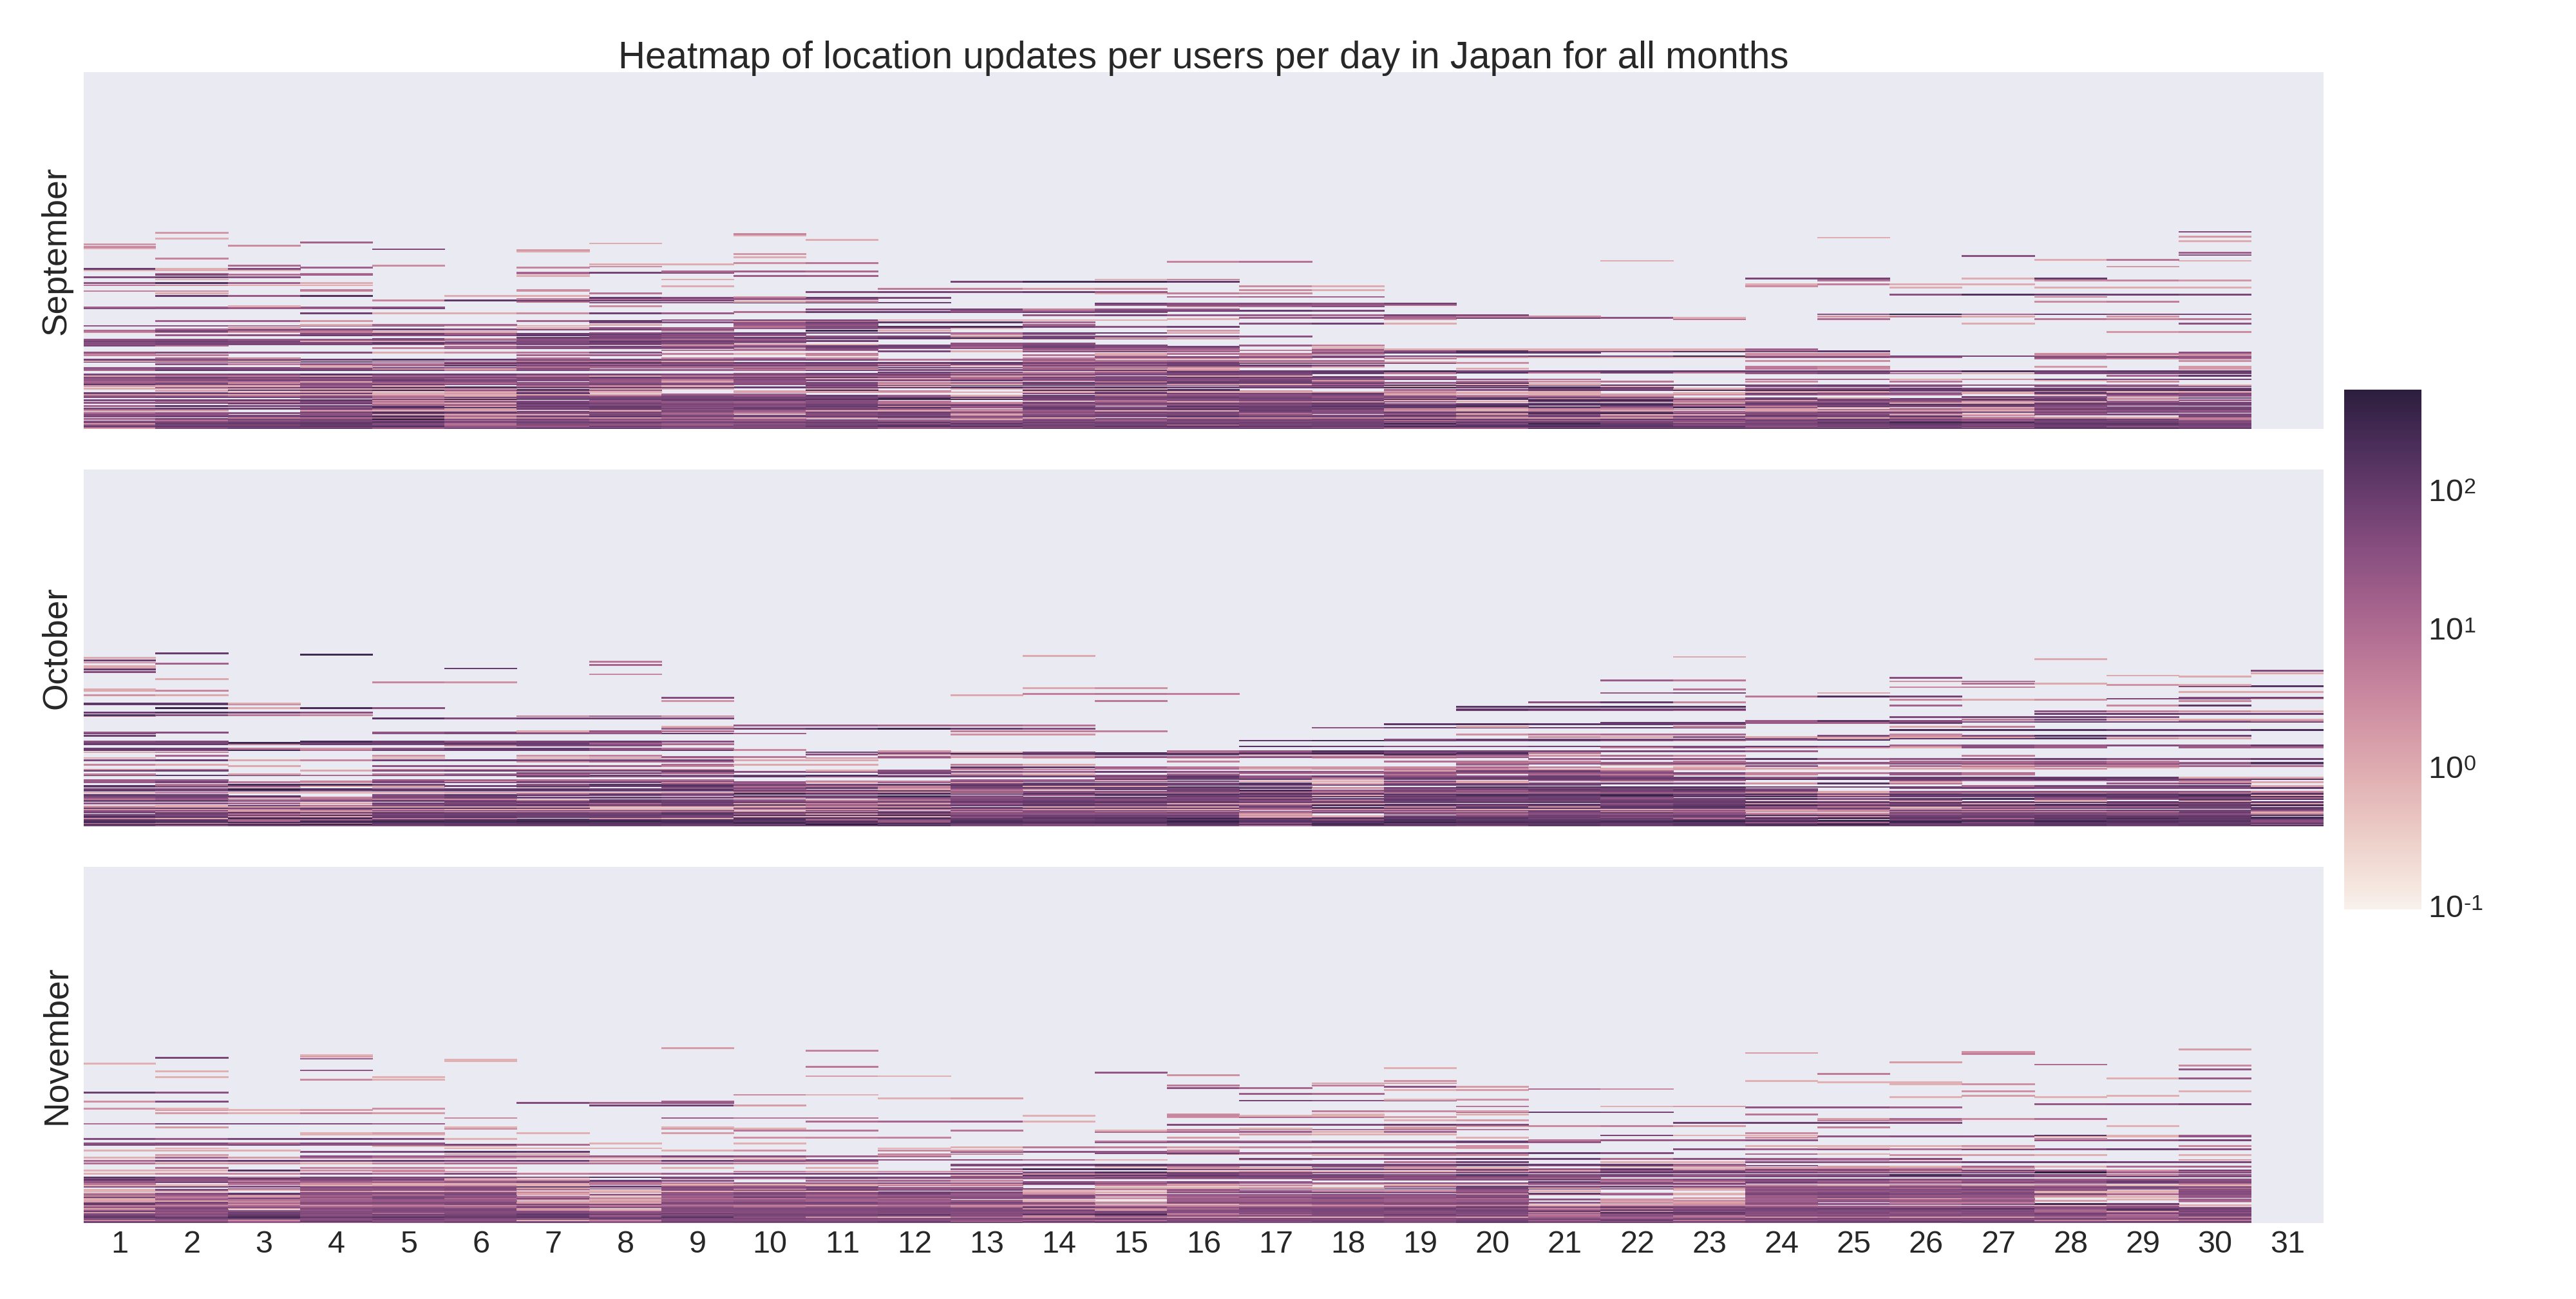
\includegraphics[scale=0.16]{location_updates_japan_combined_log.png}
    \caption{Heat map for mean location updates over the 3 month period in Japan}
    \label{fig:heatmap_japan_combined}
\end{figure}

\begin{figure}[H]
    \hspace*{-1.5cm}
    \centering
    
\includegraphics[scale=0.16]{location_updates_sweden_combined_log.png}
    \caption{Heat map for mean location updates over the 3 month period in Sweden}
    \label{fig:heatmap_sweden_combined}
\end{figure}

\begin{figure}[H]
    \hspace*{-1.5cm}
    \centering
    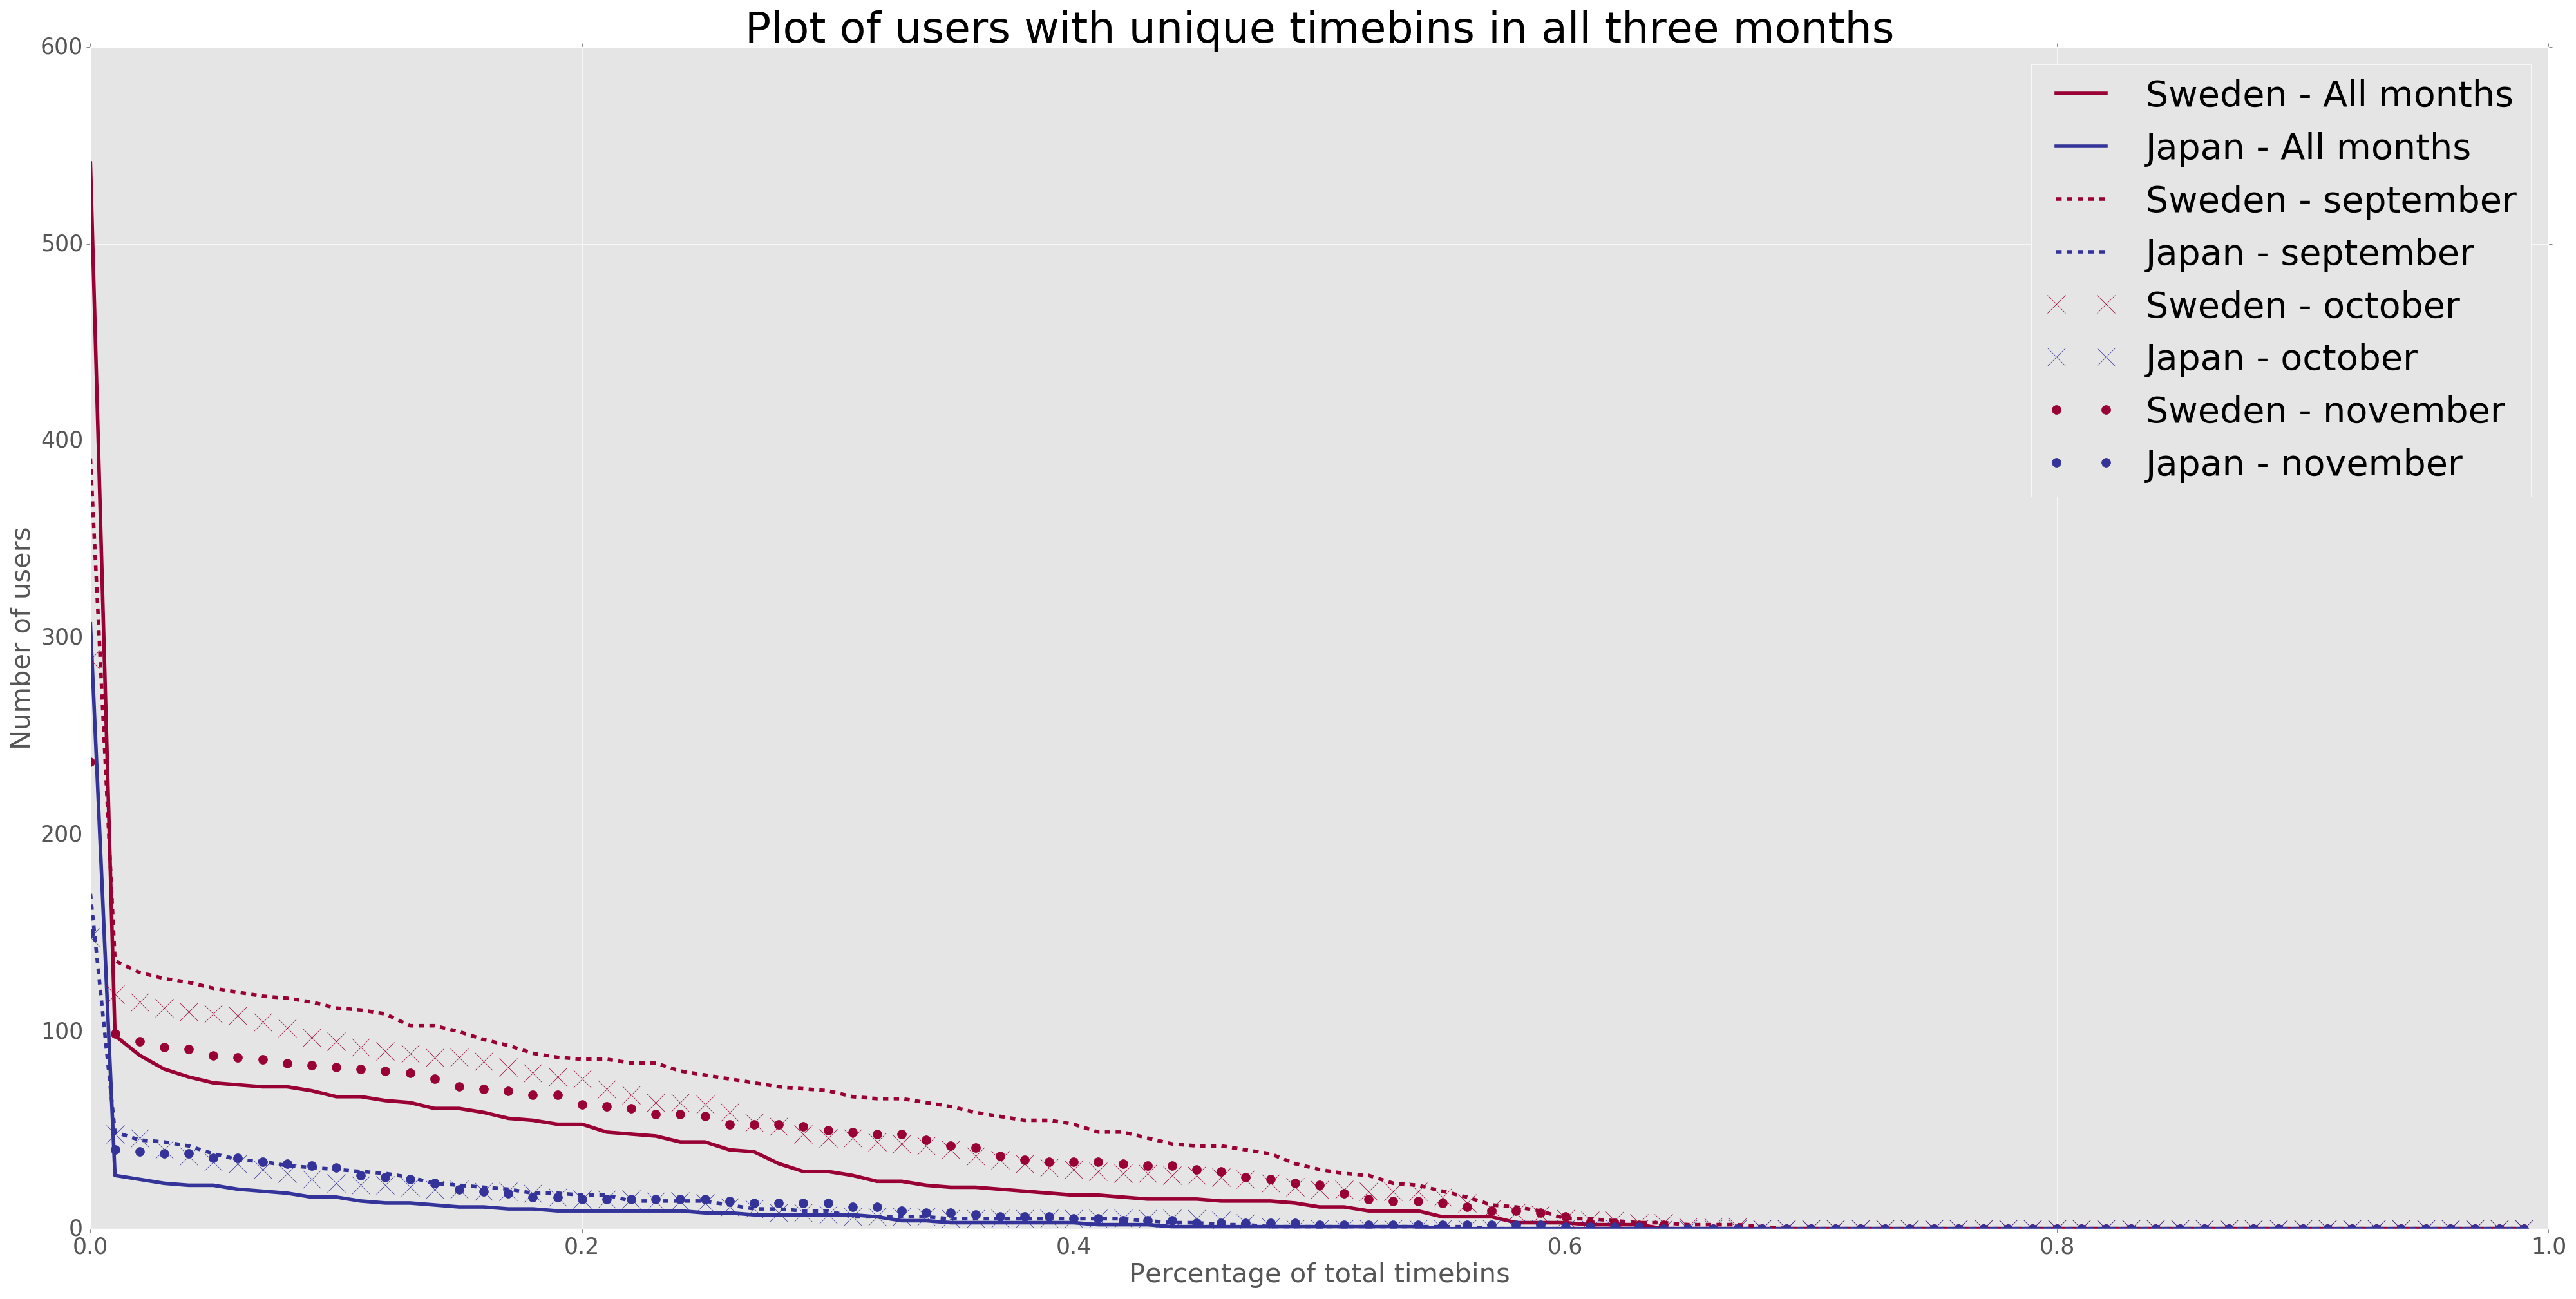
\includegraphics[scale=0.25]{users_by_criteria.png}
    \caption{}
    \label{fig:users_by_criteria}
\end{figure}

\newpage
Our work will focus on the location updates from Japan. There is 332 users in Japan for which we have location updates.
When training our classifier we divided the dataset into three parts where each corresponded to a month.

Japan locations for September: 340198
Japan locations for October: 208242
Japan locations for November: 102442


Over disse 3 måneder blev der indsamlet 2.665.893 geolokation lokations opdaterings, som er vores primær data. 

When we got the dataset it was stored in three folders, one for each month (9, 10, 11) and within each folder were multiple chunks of data in Apache Avro format\cite{apacheavro}, which we learned is a data serialization framework for Hadoop similar to the JSON format. The chunks were contained in folders bearing the number for each month, however we learned they were sorted by when the server had received the data packet containing the location from the phone and not when the phone had registered the location. The app is storing the collected data on the users phone for a maximum of one month, if the data is not uploaded within a month it is discarded. This approach to data collection means the month folders can contain location updates from the previous month as well.


\subsection{Production data}


\section{Summary}